\documentclass[aspectratio=169]{beamer}
\usetheme{mybusinessbeamertheme}

\usepackage{graphicx}
\usepackage{amsmath}
\usepackage{amsthm}
\setbeamertemplate{theorems}[numbered]
\newtheorem*{mydef}{Definition}
\newtheorem{requirement}{Req.}
\usepackage{amssymb}
\usepackage{epigraph}
\usepackage{multirow}
\usepackage{colortbl}
\usepackage{multicol}
\usepackage{eso-pic}
\usepackage{listings}
\usepackage{xcolor}
\usepackage{booktabs}
\usepackage{tikz}
\usetikzlibrary{positioning}

% Code listing style (from the data-and-information-modelling deck)
\definecolor{codebg}{HTML}{f2f5f7}
\definecolor{codecomment}{HTML}{6b7a88}
\definecolor{codekey}{HTML}{04395e}
\definecolor{codestr}{HTML}{b5651d}
\definecolor{codekw}{HTML}{70a288}
\lstdefinestyle{code}{
  basicstyle=\ttfamily\scriptsize,
  commentstyle=\color{codecomment}\itshape,
  stringstyle=\color{codestr},
  breaklines=true,
  breakatwhitespace=true,
  frame=single,
  backgroundcolor=\color{codebg},
  tabsize=2,
  showstringspaces=false,
  columns=fixed,
  xleftmargin=1.5em, xrightmargin=1em,
  framesep=3pt
}

% Colours used by the IntegratingInformationStandards slides
\definecolor{newgray}{HTML}{001D4A}
\definecolor{newdarkblue}{HTML}{27476E}
\definecolor{newmidblue}{HTML}{006992}
\definecolor{newlightblue}{HTML}{EAF8BF}
\definecolor{neworange}{HTML}{ECA400}

% Column types used by the IntegratingInformationStandards tables
\newcolumntype{a}{>{\columncolor{newlightblue}}c}
\newcolumntype{o}{>{\columncolor{neworange}}c}

\AtBeginEnvironment{requirement}{%
  \setbeamercolor{block title}{use=example text,fg=newgray}
  \setbeamercolor{block body}{parent=normal text,use=block title example,bg=newlightblue}
}

\title{Standardization, Interoperability \& Information Modelling}
\subtitle{Session 1 — what it means to define an information standard, and looking at openADR through that lens}
\author{Joep van Genuchten, uuidea}
\date{November 10, 2026}

\begin{document}

\frame{\titlepage}

\begin{frame}{whoami}
	\begin{columns}[T]
		\begin{column}{0.35\textwidth}
			
\includegraphics[width=\linewidth, height=0.55\textheight, keepaspectratio]{slides/whoami/figs/joep_headshots-lo-res-social-3.jpg}
		\end{column}

		\begin{column}{0.65\textwidth}
			\begin{itemize}
				\item \textbf{Name}: Joep van Genuchten
				\item \textbf{Position/Role}: Data Architect/Contractor
				\item \textbf{Institution/Organization}: uuidea
				\item \textbf{Interests}:
				      \begin{itemize}
					      \item Interoperability
					      \item Data and Semantics
					      \item Aligning different architectural layers
					      \item Taking architecture beyond the design phase
					      \item Open Source
				      \end{itemize}
			\end{itemize}
		\end{column}
	\end{columns}
\end{frame}

% 
\begin{frame}{Disclaimer}
	\begin{itemize}

		\item The views expressed in this presentation are my own and do not represent those of uuidea.
		\item The contents of this presentation are licensed under \href{https://creativecommons.org/licenses/by-sa/4.0/deed.en}{CC BY-SA 4.0}\pause
		\item I'm not an electrical engineer...
	\end{itemize}
\end{frame}

\begin{frame}{Overview}
  \small
  \begin{multicols}{2}
    \begin{itemize}
      \item \textbf{1 — the foundations}
      \begin{itemize}
        \item interoperability: what is actually involved
        \item SGAM: where openADR sits — \alert{in a hands-on exercise}
        \item the Ship of Theseus: identity, meaning \& MDM
        \item information modelling 101: L0--L3, RDF, SKOS, OWL, SHACL
        \item the requirements — the yardstick the rest of the day is built on
      \end{itemize}
      \item \textbf{2 — the requirements, addressed one at a time}
      \begin{itemize}
        \item Req.\ 1: kinds of information models — vocabulary vs.\ constraint
        \item Req.\ 2: MOF — metamodels, expressivity, transformation
        \item meaning: OWA/CWA, the open world
        \item Req.\ 3: ontology alignment, upper ontologies
      \end{itemize}
      \item \textbf{3 — in practice, and the lens turned back on openADR}
      \begin{itemize}
        \item profiles: use-case specific models
        \item the toolchain: Avro, JSON Schema, SQL — \emph{generated}
        \item Netbeheer Nederland: the practice
        \item the three requirements, applied to openADR 3.0
      \end{itemize}
    \end{itemize}
  \end{multicols}
\end{frame}

\begin{frame}{Glossary — the words we'll use today (1/2)}
  \framesubtitle{One table, so everyone means the same thing by the same word}
  \scriptsize
  \setlength{\tabcolsep}{4pt}
  \renewcommand{\arraystretch}{1.15}
  \begin{center}
  \begin{tabular}{@{}p{3.3cm}p{11.5cm}@{}}
    \toprule
    \textbf{Term} & \textbf{What it is}\\
    \midrule
    \textbf{Interoperability} & A \emph{community} quality: systems able to work together \emph{without modification}.\\
    \textbf{Standard} & A reference point against which other things can be evaluated or compared\\
    \textbf{Model} & Something that a copy can be based on because it is an extremely good example of its type \\
    \textbf{Information model (IM)} & The \emph{model} of a domain's information. abbreviated \emph{IM}.\\
    \textbf{Business Terms} & The natutal language definitions of the things we talk about.\\
    \textbf{Vocabulary Model} & information model that relies on set theoretical semantics to describe a domain. Built on the \emph{open} world; reusable across use cases\\
    \textbf{Constraint model} & The \emph{data structure} of a use case: what fields exist and how much of each; built on the \emph{closed} world.\\
    \textbf{Profile} & A reference to an information model \emph{plus} added constraints (scope, cardinality, value-space).\\
    \textbf{Serialization} & A concrete \emph{exchange format} for a specific pattern: Avro, JSON Schema, SQL DDL. Also called \emph{schema} or \emph{artifact} (L3).\\
    \textbf{Meta-model} & A model \emph{of} models (UML, OWL, SHACL, JSON Schema\ldots).\\
    \textbf{Meta-meta-model} & A model of meta-models (MOF, RDF/S).\\
    \textbf{Pivot model} & A chosen meta-model with enough expressivity to transform to and from the others.\\
    \bottomrule
  \end{tabular}
  \end{center}
\end{frame}

\begin{frame}{Glossary — the words we'll use today (2/2)}
  \framesubtitle{One table, so everyone means the same thing by the same word}
  \scriptsize
  \setlength{\tabcolsep}{4pt}
  \renewcommand{\arraystretch}{1.15}
  \begin{center}
  \begin{tabular}{@{}p{3.3cm}p{11.5cm}@{}}
    \toprule
    \textbf{Term} & \textbf{What it is}\\
    \midrule
    \textbf{Ontology} & A formal, machine-interpretable account of meaning and relationships (ISA, disjointness) --- the terms other standards can align to.\\
    \textbf{Upper ontology} & A high-level classification of reality (BFO, nen-2660) used as a common yardstick to spot semantic conflicts.\\
    \textbf{Alignment / mapping} & A documented, reviewable link between two models' terms (\texttt{owl:equivalentClass}, \texttt{skos:closeMatch}).\\
    \textbf{SGAM} & Smart Grid Architecture Model: Business / Function / Information / Communication / Component layers.\\
    \textbf{CIM / CGMES} & IEC 61970 CIM is the energy \emph{vocabulary}; CGMES is the ENTSO-E profile on top of it.\\
    \textbf{mRID} & A globally unique, persistent identifier (IEC 61970-552) that survives change.\\
    \bottomrule
  \end{tabular}
  \end{center}
\end{frame}


\section{What interoperability is — and what it takes}
\subsection{Interoperability — what!?}\label{subsec:Definitions}
\begin{frame}{Interoperability — what!?}
  \begin{definition}{Merriam Webster}
    \small \textit{in·ter·op·er·a·bil·i·ty} — ability of a system (such as a weapons system) to work with or use the parts or equipment of another system.
  \end{definition}

  \begin{definition}{Cambridge Dictionary}
    \small Interoperability: the degree to which two products, programs, etc.\ can be used together, or the quality of being able to be used together.
  \end{definition}

  \vspace{0.3cm}
  \begin{center}
    {\large As a data architect, I love me some well-defined terms!}
  \end{center}
\end{frame}

\begin{frame}{Interoperability — what!? (2)}
  \begin{definition}{U.S. Department of Energy}
    \small Interoperability: the ability of systems, personnel, or organizations to provide services to and accept services from other systems, personnel, or organizations, and to use the services so exchanged so that these organizations can operate together effectively.
  \end{definition}

  \vspace{0.3cm}
  \begin{definition}{Red Hat}
    \small Interoperability: the connection of data, applications, APIs, and devices across your IT organization to be more efficient, productive, and agile.
  \end{definition}
\end{frame}

\subsection{Interoperability — what!?}\label{subsec:ConverterBox}
\begin{frame}{Interoperability — what!?}
  \begin{center}
    \includegraphics[height=0.4\textwidth]{slides/context/converter-box/figs/converter-box.png}\\[0.5cm]
    {\large Wait\ldots{} what!? This is interoperability?}
  \end{center}
\end{frame}

\subsection{Interoperability — what!?}\label{subsec:ConnectorCables}
\begin{frame}{Interoperability — what!?}
  \begin{center}
    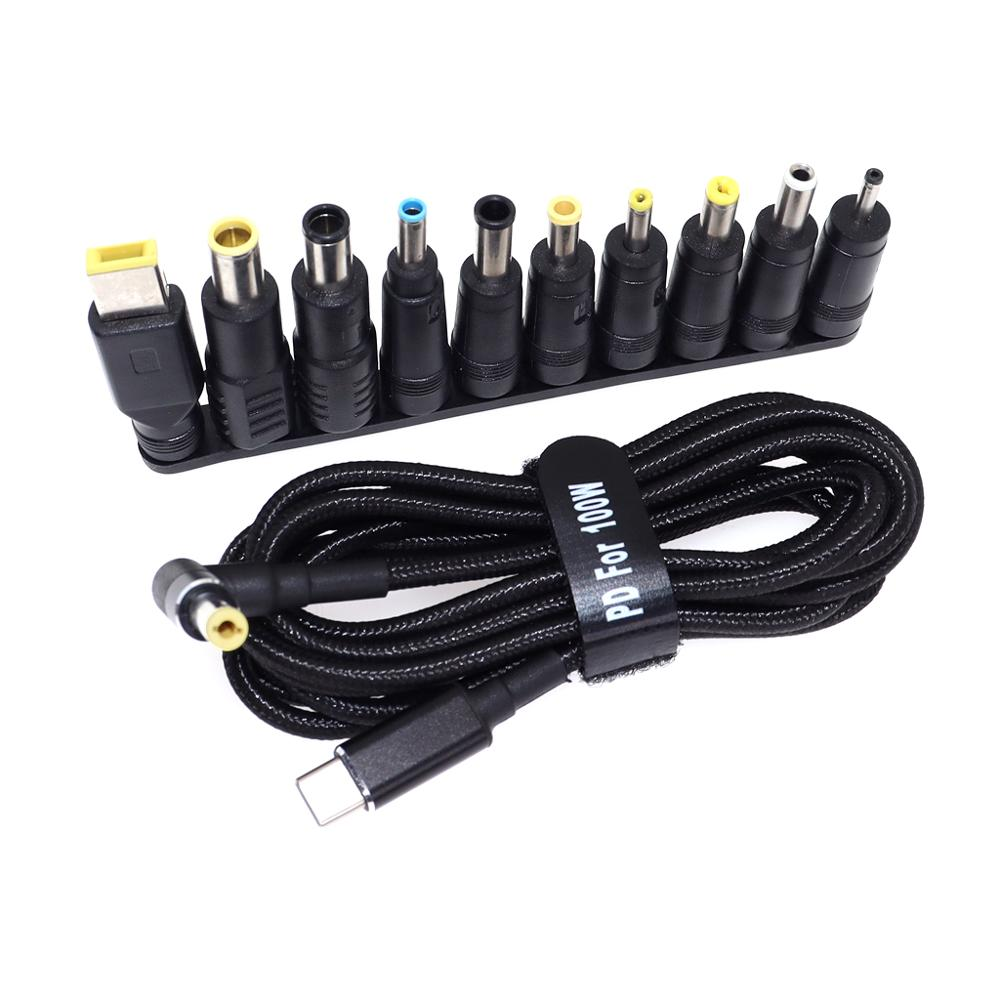
\includegraphics[height=0.45\textheight]{slides/context/cables/figs/cable-adapters.jpeg}%
    \qquad
    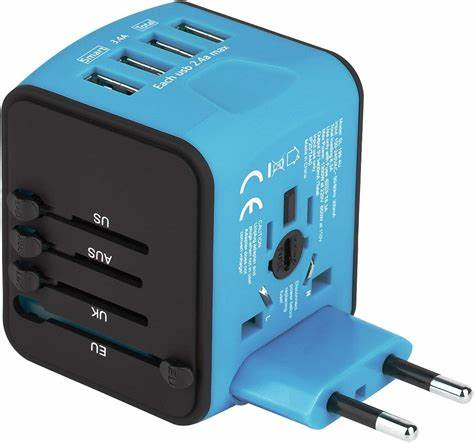
\includegraphics[height=0.45\textheight]{slides/context/cables/figs/travel-charger.jpeg}
  \end{center}
\end{frame}

\subsection{Interoperability — what!?}\label{subsec:IntegrationVsInteroperability}
\begin{frame}{Interoperability — what!?}
  \begin{center}
    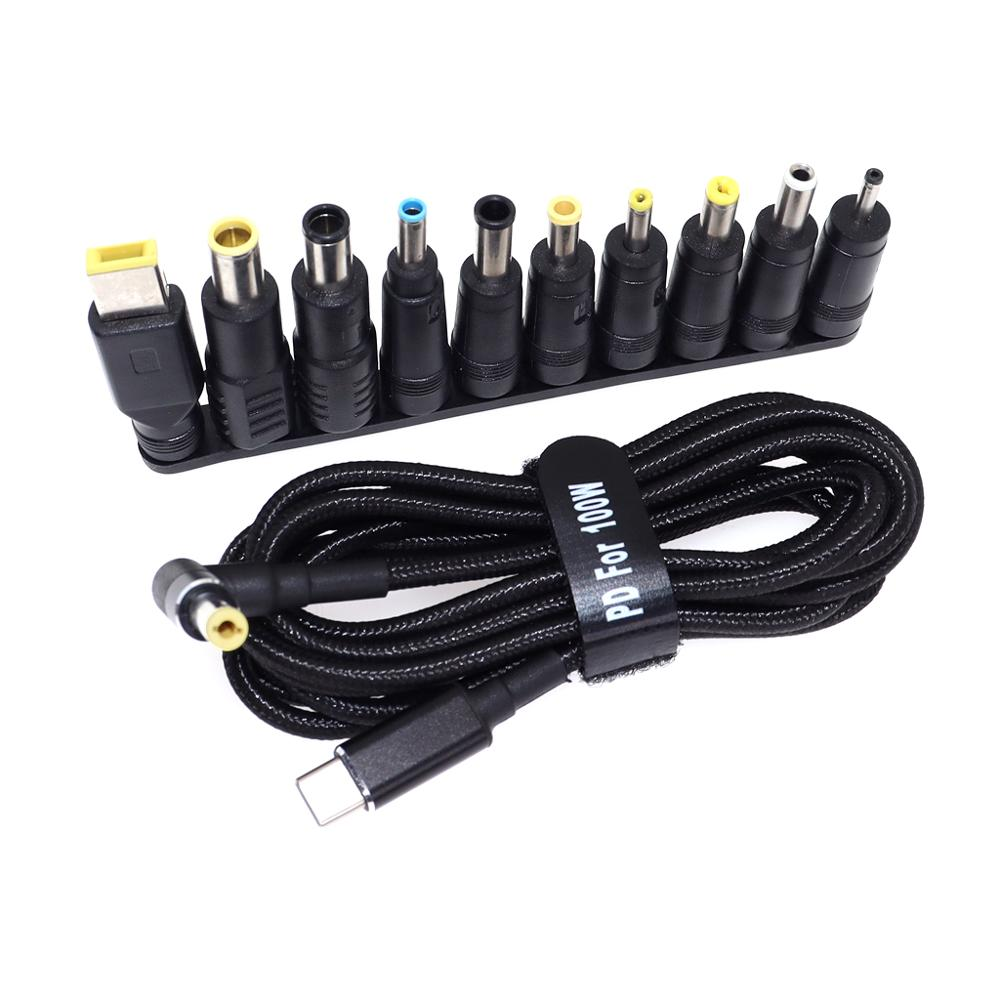
\includegraphics[height=0.32\textheight]{slides/context/cables/figs/cable-adapters.jpeg}%
    \qquad
    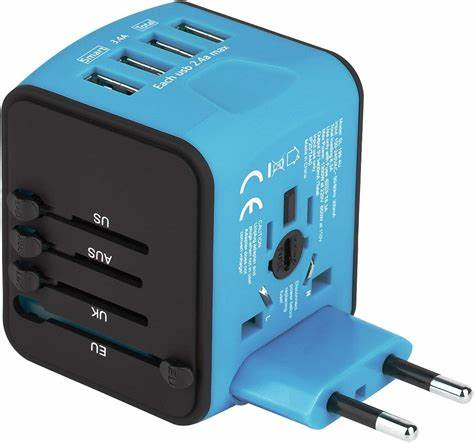
\includegraphics[height=0.32\textheight]{slides/context/cables/figs/travel-charger.jpeg}
  \end{center}

  \vspace{0.4cm}
  \begin{center}
    {\large\itshape Upon further reflection:}
  \end{center}
  \vspace{0.3cm}
  \begin{alertblock}{}
    When systems can work together but have been \emph{modified} to do so, they are \alert{integrated}.
    \vspace{0.2cm}
    \small Merriam Webster: $[\,$systems that are$\,]$ designed to work with another device or system \emph{without modification} $[\,$are compatible$\,]$.
  \end{alertblock}
\end{frame}

\subsection{Interoperability — what!?}\label{subsec:USBc}
\begin{frame}{Interoperability — what!?}
  \begin{block}{EU legislation}
    \small Requires Apple (and all other smartphone manufacturers) to use \textbf{USB-C} for the data/charging interface.
    Motivation: the need for interoperability to reduce e-waste and increase customer choice of vendors.
  \end{block}

  \vspace{0.4cm}
  \begin{definition}{Compatible}
    \small Designed to work with another device or system \emph{without modification} (Merriam Webster).
  \end{definition}

  \vspace{0.4cm}
  \begin{center}
    {\LARGE\alert{We need standards!}}
  \end{center}
\end{frame}

\subsection{Interoperability — what!?}\label{subsec:StandardsProliferation}
\begin{frame}{Interoperability — what!?}
  \begin{columns}[T]
    \begin{column}{0.5\textwidth}
      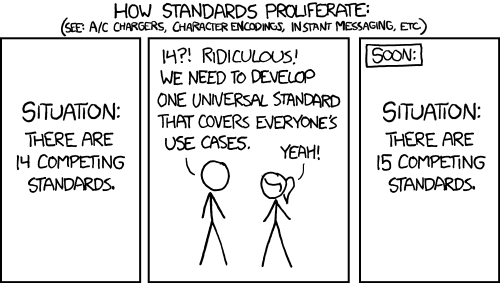
\includegraphics[width=\linewidth]{slides/context/standards-proliferation/figs/standards-proliferation.png}
    \end{column}
    \begin{column}{0.5\textwidth}
      \includegraphics[width=\linewidth]{slides/context/standards-proliferation/figs/converter-box.png}
    \end{column}
  \end{columns}

  \vspace{0.4cm}
  \begin{center}
    {\large All of these are standards\ldots{} so that is not enough either.}
  \end{center}
\end{frame}

\subsection{The importance of communities}\label{subsec:CommunitiesSolo}
\begin{frame}{The importance of communities in the pursuit of interoperability}
  \begin{center}
    \begin{tikzpicture}[
      bubble/.style={draw=primary, rounded corners=12pt, fill=tertiary!15,
                     font=\small, inner sep=8pt, align=center}
    ]
      \node (a) at (0,0)
        {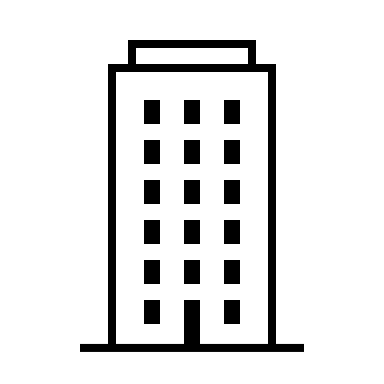
\includegraphics[width=2.6cm]{slides/context/communities/figs/organization-a.png}};
      \node [bubble, above=0.2cm of a] {``I am sooo interoperable''};

      \node (b) at (5.5,0)
        {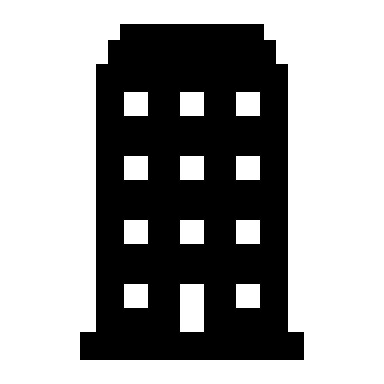
\includegraphics[width=2.6cm]{slides/context/communities/figs/organization-b.png}};
      \node [bubble, above=0.2cm of b] {``No! \alert{I} am sooo interoperable''};
    \end{tikzpicture}
  \end{center}

  \vspace{0.5cm}
  \begin{center}
    {\large\itshape Two organizations — each claiming interoperability, with no one to interoperate with.}
  \end{center}
\end{frame}

\subsection{The importance of communities}\label{subsec:CommunitiesTogether}
\begin{frame}{The importance of communities in the pursuit of interoperability}
  \begin{center}
    \begin{tikzpicture}[
      bubble/.style={draw=primary, rounded corners=12pt, fill=accent!25,
                     font=\small, inner sep=8pt, align=center}
    ]
      \node (a) at (0,0)
        {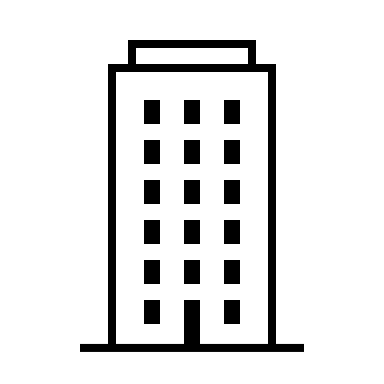
\includegraphics[width=2.6cm]{slides/context/communities/figs/organization-a.png}};
      \node [bubble, above=0.2cm of a] {``\alert{We are} sooo interoperable''};

      \node (b) at (5.5,0)
        {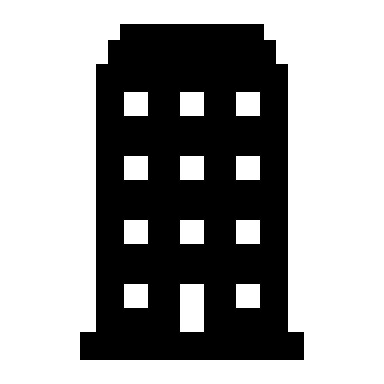
\includegraphics[width=2.6cm]{slides/context/communities/figs/organization-b.png}};
      \node [bubble, above=0.2cm of b] {``\alert{We are} sooo interoperable''};
    \end{tikzpicture}
  \end{center}

  \vspace{0.5cm}
  \begin{center}
    {\large\itshape Interoperability is a quality of a community of contributors.}
  \end{center}
\end{frame}


\section{SGAM and where openADR lives on it}
\begin{frame}{SGAM Refresher}
	\begin{figure}
		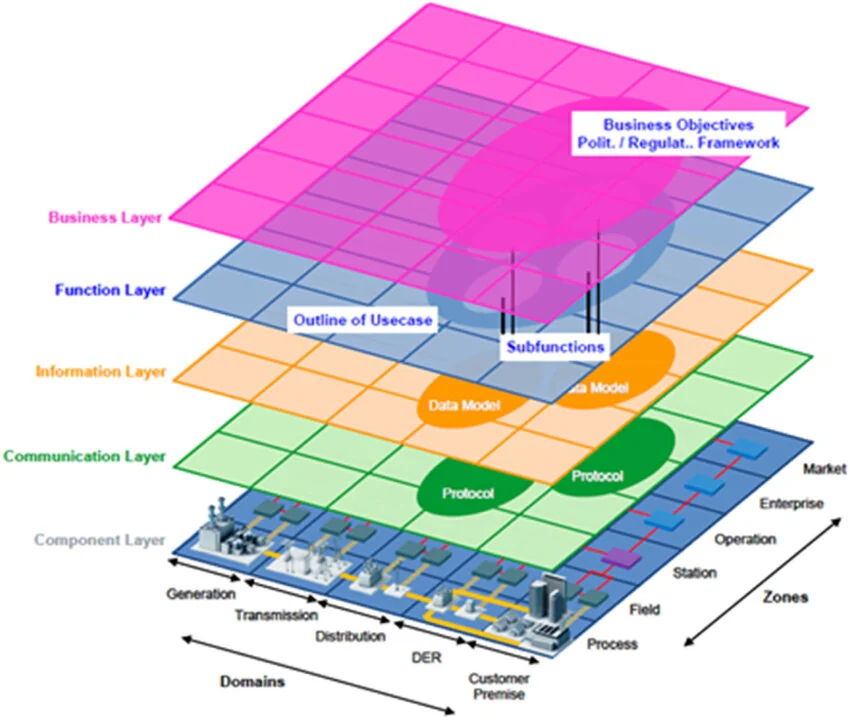
\includegraphics[height=0.72\textheight]{slides/sgam/figs/sgam-refresher-der.png}
	\end{figure}
\end{frame}

\begin{frame}{SGAM: the layers}

  \begin{table}
    \begin{tabular}{lp{11cm}}
      \rowcolor[HTML]{031d44}
      {\color{white}\textbf{Layer}} & {\color{white}\textbf{Question it answers}} \\
      \textbf{Business} & Why do we exist? What capabilities do we have? \\
      \textbf{Function} & How do we achieve our capabilities, what is the process? \\
      \textbf{Information} & What information is exchanged for the purpose of the process? \emph{mean}? \\
      \textbf{Communication} & How do we transmit it? Integration patterns, protocols, etc \\
      \textbf{Component} & What physical/digital artifacts run it? Software, hardware, platforms. \\
    \end{tabular}
  \end{table}

  \vspace{0.3cm}
  \begin{alertblock}{Key point}
    Interoperability failures usually happen\emph{cross-layer}: you agree on the protocol, but not on what the bytes \emph{mean} — or on what the business process requires.
  \end{alertblock}
\end{frame}

\begin{frame}{Exercise: plot openADR on the SGAM framework}
  \framesubtitle{Working exercise — \textasciitilde{}20 minutes, in pairs}

  \begin{enumerate}
    \item Take the openADR building blocks you know best:
      % \begin{itemize}
      %   \item a DER / flexibility resource, its capabilities and set-points
      %   \item the openADR protocol \& message types (offer, order, status)
      %   \item the roles: DSO, aggregator, DER owner, market party
      %   \item the use cases: congestion management, frequency response, peak shaving
      %   \item the systems: grid systems, BMS/PMS, market platforms, devices
      % \end{itemize}
    \item Place each of them on the domains and zones  
    \item Place each of them on the SGAM layers:
      \alert{Business \textbar{} Function \textbar{} Information \textbar{} Communication \textbar{} Component}
    % \item For each placement, write one sentence: \emph{what do we actually agree on at this layer?}
  \end{enumerate}

  \vspace{0.3cm}
  \begin{block}{Deliverable}
    Draw out the zones/dimensions grid and plot your building block on the grid and describe each layer in terms of your block/usecase
  \end{block}
\end{frame}

% \begin{frame}{Exercise debrief: what a mapping might look like}
  \framesubtitle{A sketch — not one single right answer}

  \begin{table}
    \begin{tabular}{lp{11cm}}
      \rowcolor[HTML]{dab785}
      {\color{newgray}\textbf{SGAM layer}} & {\color{newgray}\textbf{openADR material on that layer}} \\
      Business & Flexibility product as market offering; congestion relief as service; value = avoided investments, reliability \\
      Function & Bidding/set-pointing loop; capacity calculation; dispatching orders; settlement \& reporting \\
      Information & \alert{Capabilities, set-points, actuals, status, identities (who/what/where)} — \emph{where is the shared model?} \\
      Communication & openADR (REST/JSON), transport, security (OAuth), messaging semantics \\
      Component & Devices (chargers, BMS), DER controller, DSO grid system, aggregator platform \\
    \end{tabular}
  \end{table}

  \vspace{0.2cm}
  \pause
  What usually shows up: strong \textbf{Business/Function/Communication}, thin \textbf{Information}.
  That thinness is exactly where Day 2 lives.
\end{frame}

% \begin{frame}{Looking ahead}
  % \framesubtitle{And why the rest of this week is about it}
  \footnotesize
  \setlength{\itemsep}{1pt}
  \setlength{\parsep}{0pt}

  \begin{itemize}
    \item openADR is, structurally, a \textbf{Communication- and Function-layer} technology: messages, roles, processes, systems.
    \begin{itemize}
      \item Agreements there are \emph{protocol-level}: endpoint, format, sequence, security.
    \end{itemize}
    \pause
    \item The DSO sits on top of a large existing information layer: \alert{CIM, CGMES, IEC 61850, grid data models}.
    \begin{itemize} 
      \item openADR assets (chargers, PV, storage) will be \emph{inside} that layer as soon as they matter for grid calculations — and Day 2 starts there.
    \end{itemize}
    \pause
    \item The \textbf{Information layer is where openADR is thinnest}:
    \begin{itemize}
      \item The information standardization in which openADR finds itself is quite nuanced.
      \item In order to achieve interoperability with adjacent systems, openADR will have to adopt that nuance
    \end{itemize}

  \end{itemize}

  \vspace{0.15cm}
  \begin{alertblock}{The week's thesis}
    \emph{openADR tells DER what to do; CIM/CGMES tell everyone what the grid \emph{is}. You need both — and a bridge between them.}
    \vspace{0.1cm}
    \alert{Today's goal:} \textbf{understand what it takes to design an information standard that aligns with adjacent standards.} 
  \end{alertblock}
\end{frame}


\section{The Ship of Theseus, master data, and meaning}
\begin{frame}{The Ship of Theseus}
  \setlength{\intextsep}{0.5em}

  \only<1>{
    \begin{figure}
      \centering
      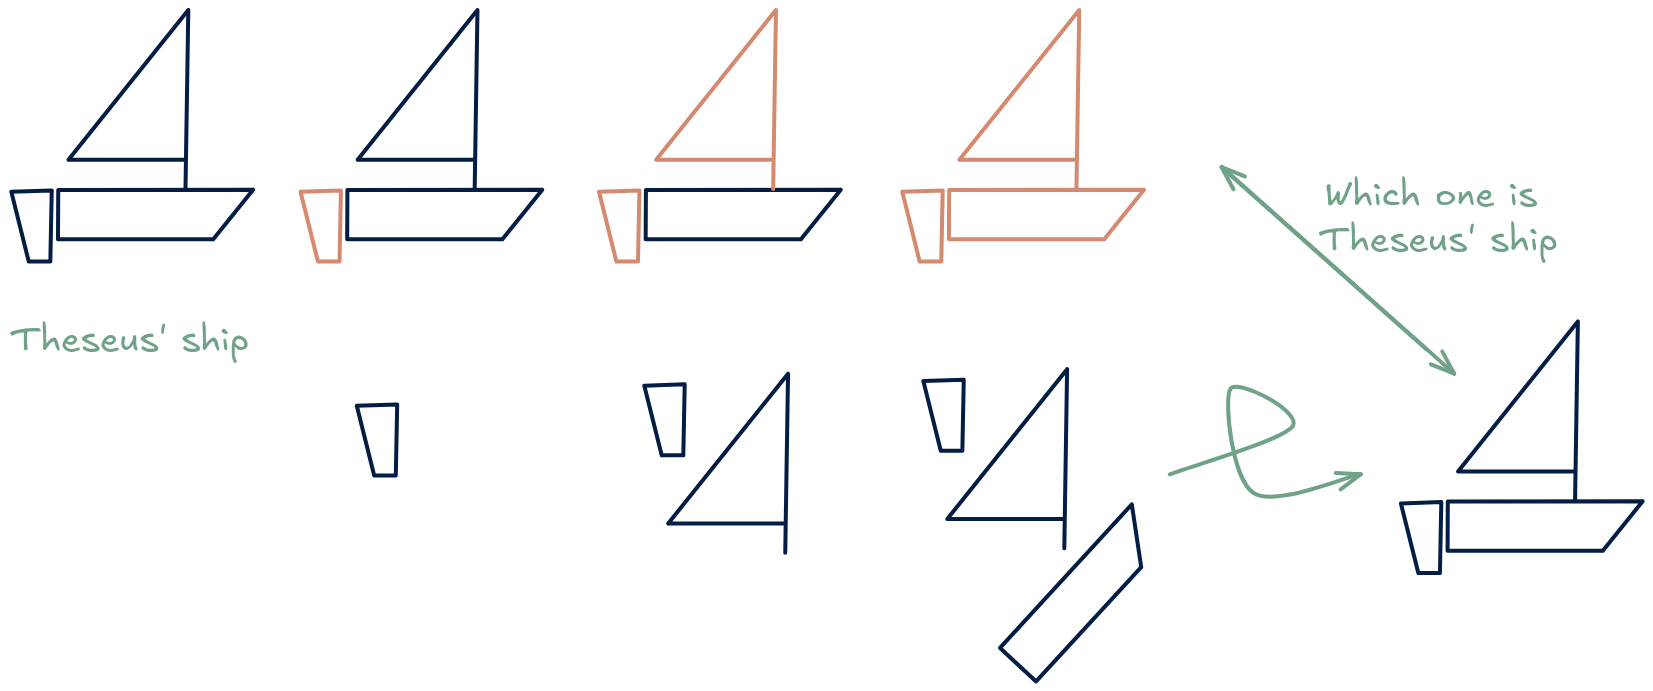
\includegraphics[width=0.85\textwidth, height=0.65\textheight, keepaspectratio]{slides/theseus/paradox/figs/ship-of-theseus-1.png}
      \caption{Planks replaced one by one, spare parts assembled into a second ship.}
    \end{figure}
  }

  \only<2>{
    \begin{figure}
      \centering
      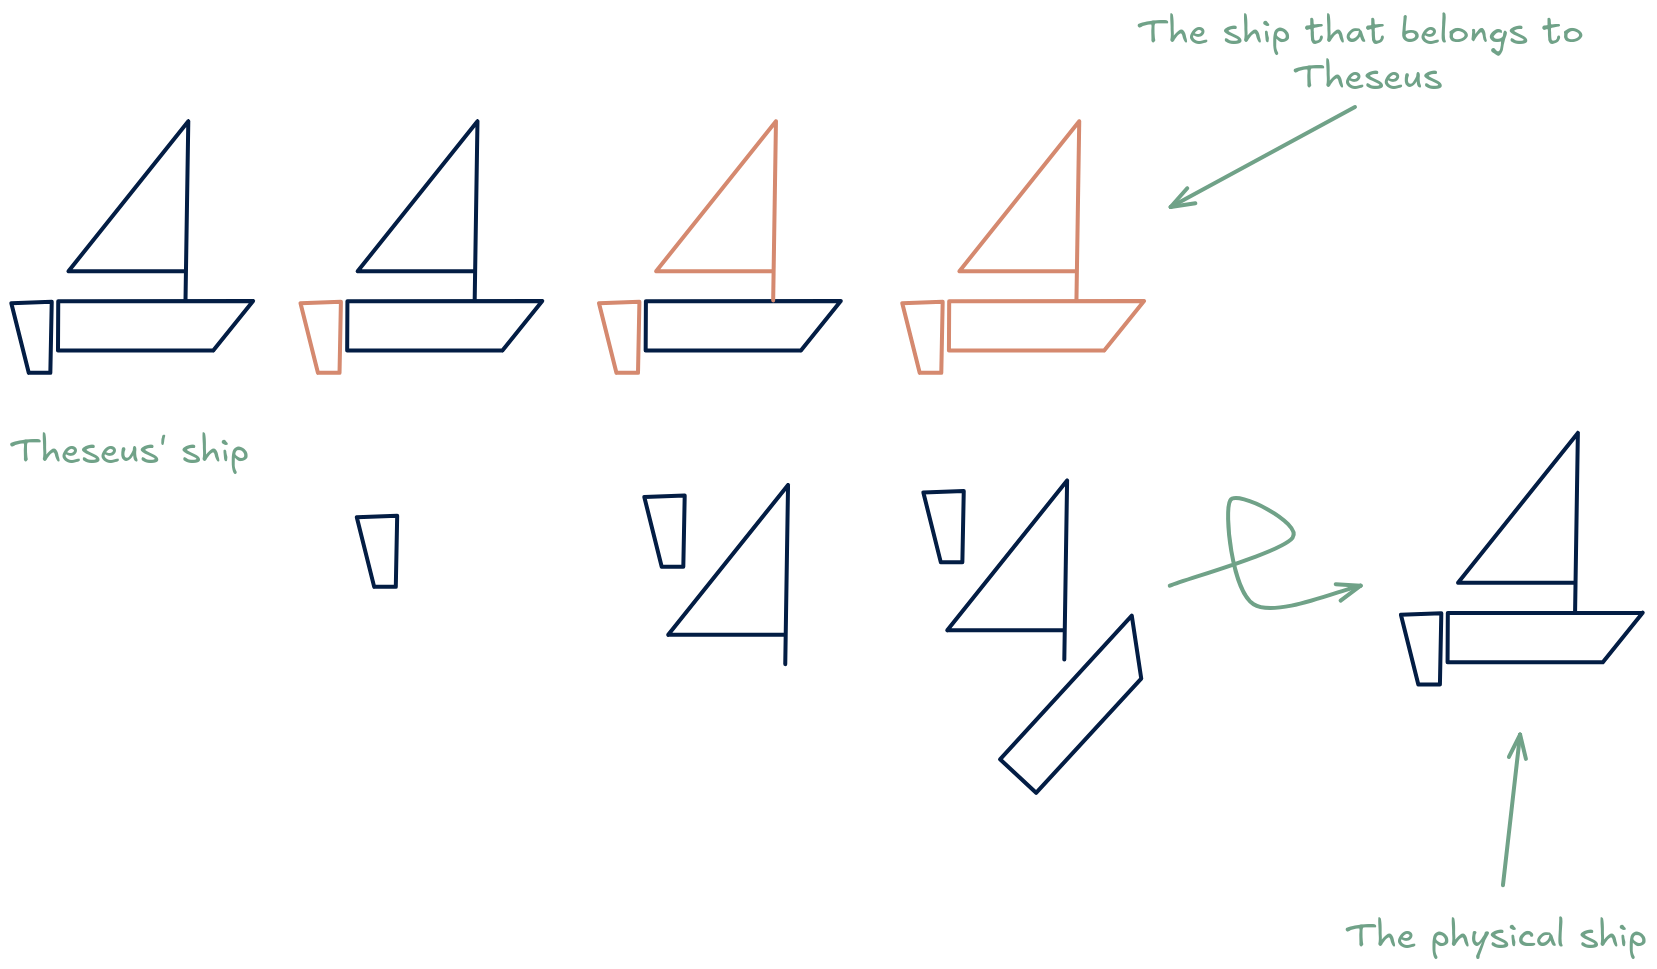
\includegraphics[width=0.85\textwidth, height=0.65\textheight, keepaspectratio]{slides/theseus/paradox/figs/ship-of-theseus-2.png}
      \caption{Two perspectives: the ship that \emph{belongs} to Theseus, and the \emph{physical} ship made of the original planks.}
    \end{figure}
  }

  \only<3>{
    \begin{figure}
      \centering
      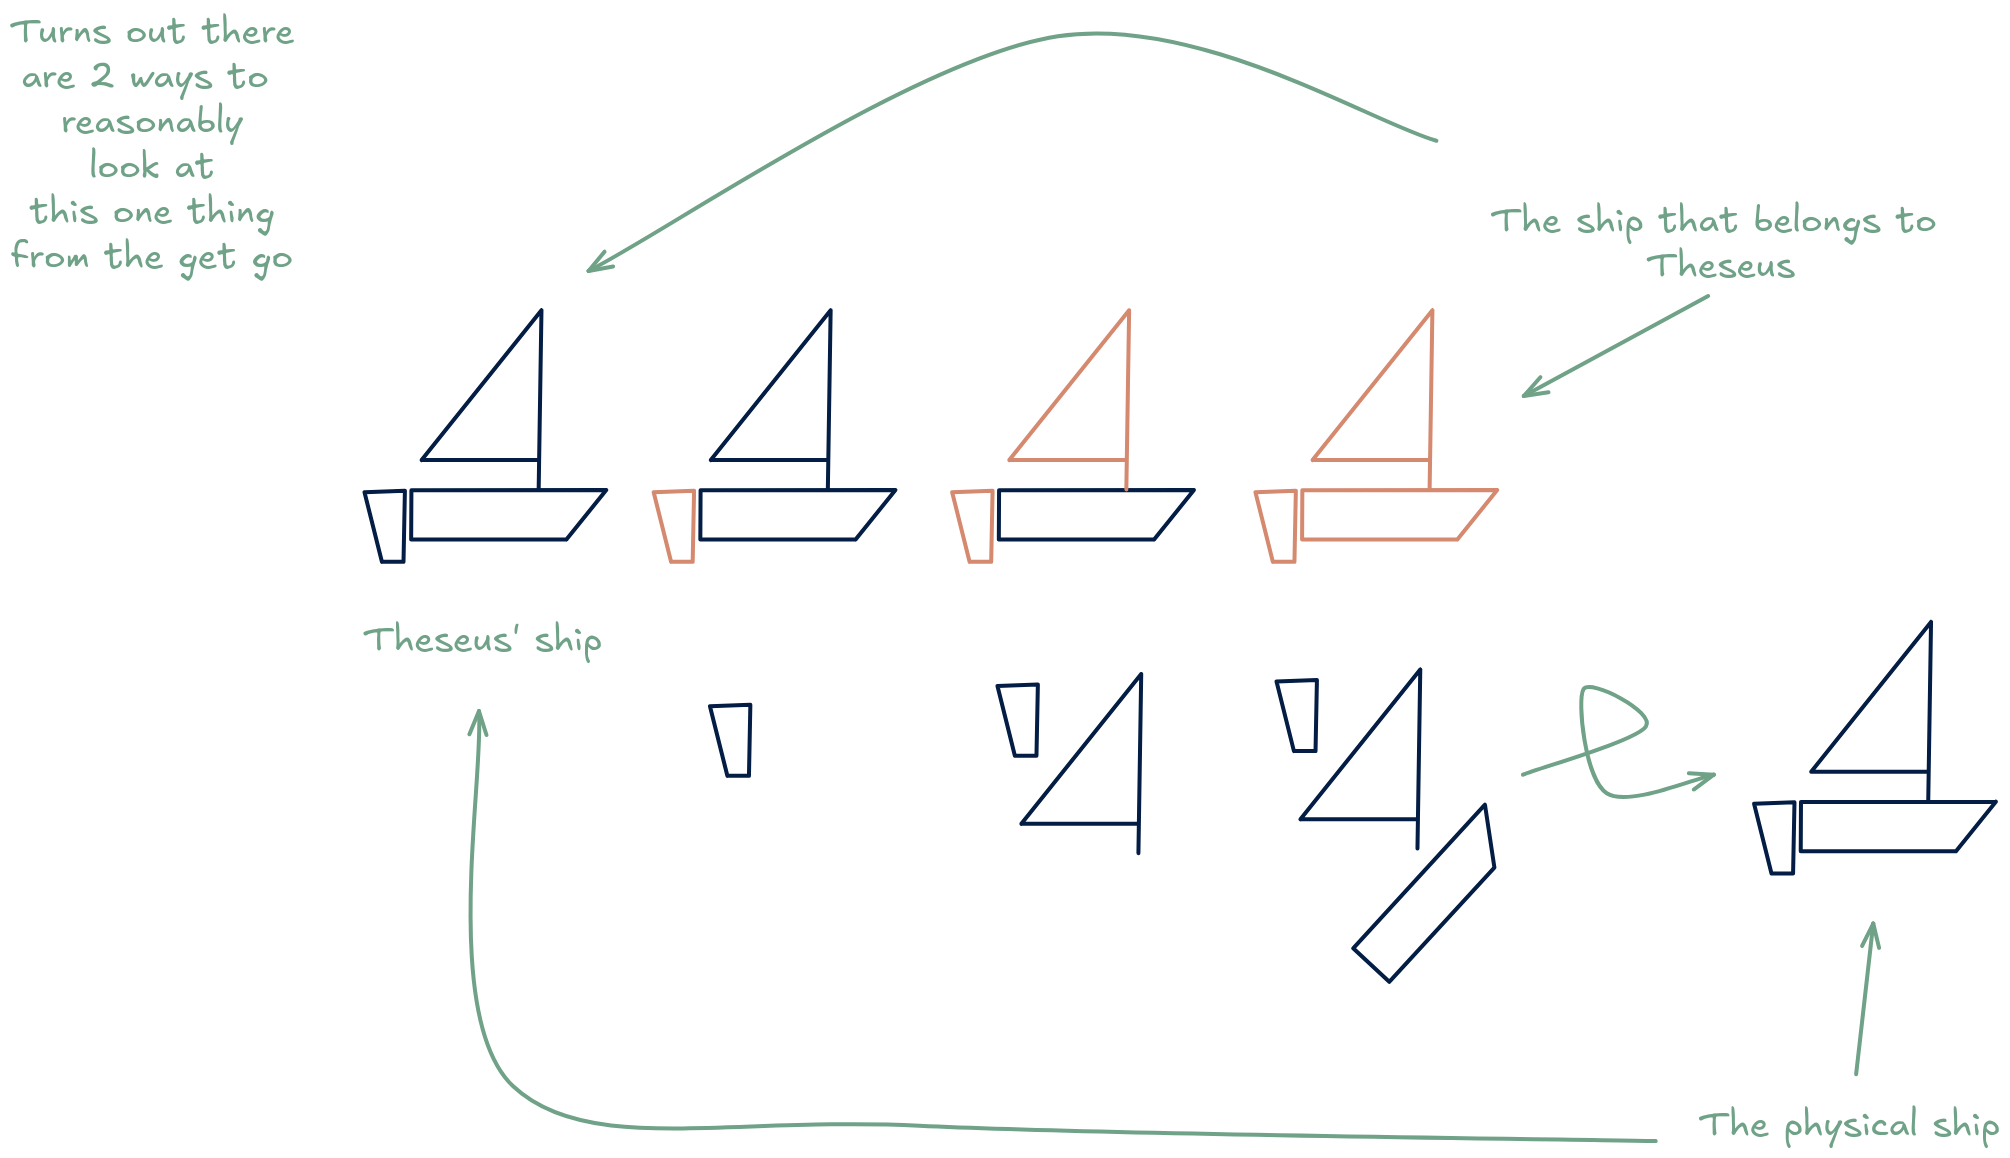
\includegraphics[width=0.85\textwidth, height=0.65\textheight, keepaspectratio]{slides/theseus/paradox/figs/ship-of-theseus-3.png}
      \caption{Turns out there are two (or more) ways to reasonably look at this one thing — from the get-go.}
    \end{figure}
  }
\end{frame}

\begin{frame}{Market services add an extra layer of interpretation}
  \setlength{\intextsep}{0.5em}

  \begin{figure}
    \centering
    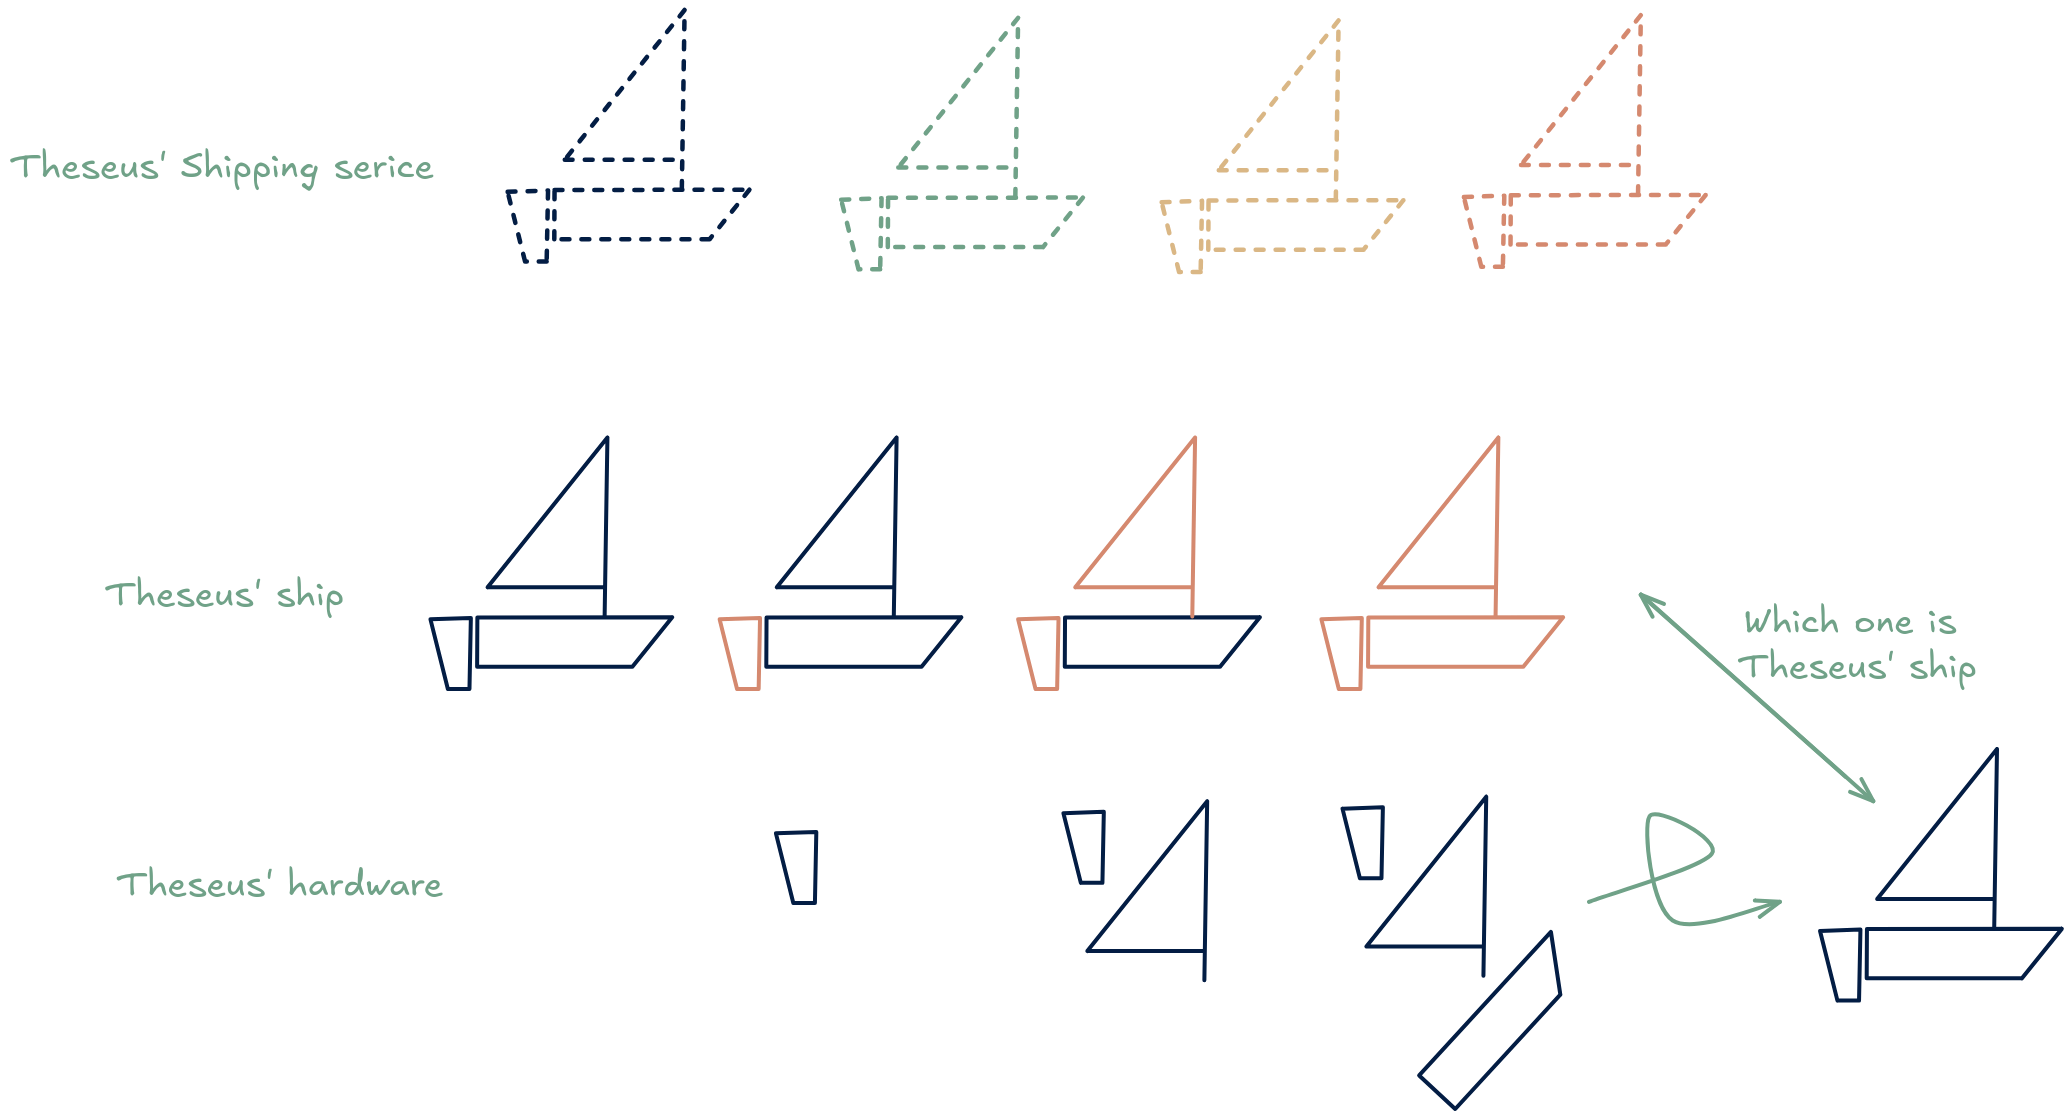
\includegraphics[width=0.85\textwidth, height=0.65\textheight, keepaspectratio]{slides/theseus/paradox/figs/shipping-service-of-theseus.png}
    \caption{Three levels of the ship of \emph{Theseus}: the shipping service, the ship, and the hardware — and still the question ``which one is Theseus' ship?''}
  \end{figure}
\end{frame}

\begin{frame}{Master data \& meaning: what actually has to be stable?}
  \footnotesize
  \setlength{\itemsep}{1pt}
  \setlength{\parsep}{0pt}

  The ship, the shipping
  service, the hardware... which one are we talking about when we refer to \emph{the ship}? and if that is unclear, what does 'ship' actually \emph{mean}?


\end{frame}


\section{Information modelling 101}
\begin{frame}{The layer model (L0--L3)}
	\small
	\begin{columns}[T]
		\begin{column}{0.62\textwidth}
			\centering
			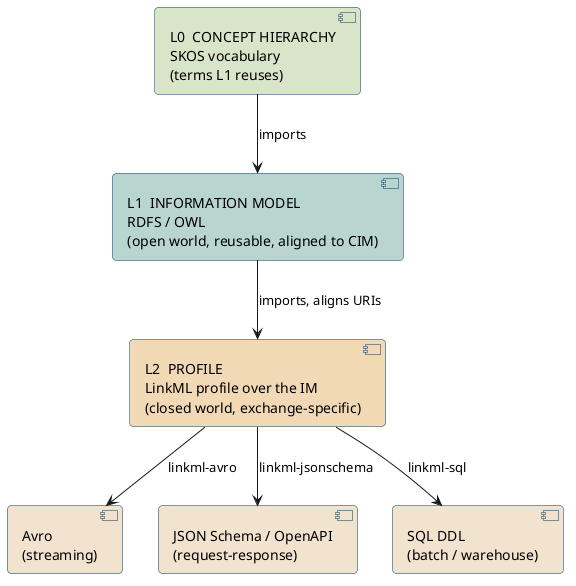
\includegraphics[width=\linewidth, height=0.46\textheight, keepaspectratio]{slides/im-101/three-layers/figs/uml-fourlayers.png}
		\end{column}
		\begin{column}{0.38\textwidth}
			\textbf{L0 Concept hierarchy}\\
			SKOS: the terms L1 reuses\\[0.45em]
			\textbf{L1 Information Model}\\
			open world, reusable, normative definitions\\[0.45em]
			\textbf{L2 Profile}\\
			closed world, \emph{adds constraints}\\[0.45em]
			\textbf{L3 Serializations}\\
			schema of a specific exchange pattern\\[0.7em]
			\color{gray}\textbf{L4 Instance data}\\
			\color{gray}record, row, JSON doc --- \emph{mostly out of scope}
		\end{column}
	\end{columns}
	\vspace{0.4em}
	\textit{Direction of authority: L0 $<$ L1 $<$ L2 $\vdash$ L3.}\\
	Never edit an artifact; edit the model above it and regenerate.
\end{frame}
\begin{frame}{Where we stand: NORA/MIM + the W3C stack}
	\small
	MIM (\emph{Metamodel voor Informatiemodellen}) — NORA's Informatielaag —
	splits modelling into five types; in this deck they are L0--L4, and we cover L0--L3.
	\vspace{0.3em}
	\footnotesize
	\setlength{\tabcolsep}{3pt}
	\begin{center}
	\begin{tabular}{@{}p{2.7cm}p{3.2cm}p{4.4cm}@{}}
		\toprule
		\textbf{MIM type} & \textbf{W3C / formalism} & \textbf{In this deck}\\
		\midrule
		Model van begrippen & \textbf{SKOS} vocabulaire & \textbf{L0} Concept hierarchy\\
		\midrule
		Conceptueel informatiemodel & \textbf{RDFS} + \textbf{OWL} & \textbf{L1} Information Model\\
		Logisch informatiemodel & \textbf{SHACL} constraints & \textbf{L2} Profile\\
		Fysiek / technisch gegevensmodel & \textbf{schema}: Avro, JSON-Schema, SQL & \textbf{L3} Serializations\\
		\midrule
		\color{gray}Registraties & \color{gray}instance = record, row, JSON doc & \color{gray}\textbf{L4} runtime data --- \emph{mostly out of scope}\\
		\bottomrule
	\end{tabular}
	\end{center}
	\vspace{0.3em}
	\small
	The \emph{model van begrippen} is our L0 — a \emph{SKOS} vocabulary:
	``\emph{een vocabulaire is geen informatiemodel}'' —
	terms we \emph{reuse}, not design.
\end{frame}

\begin{frame}{RDF — the triple}
  \framesubtitle{Everything is \texttt{subject} \texttt{predicate} \texttt{object}}

  \vspace{0.3em}
  \centering
  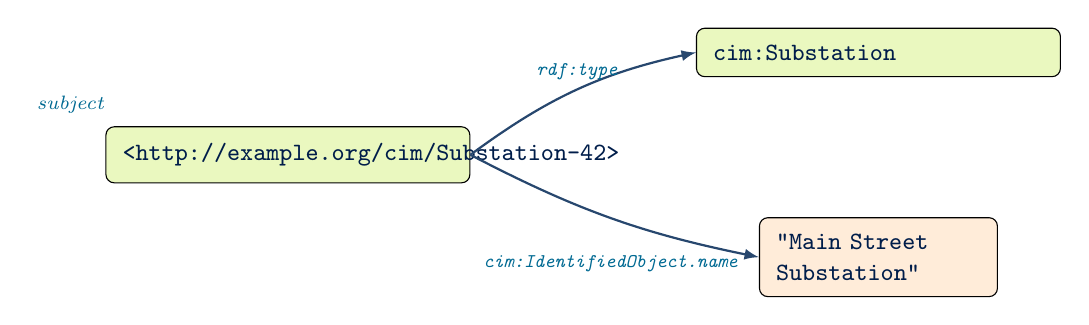
\begin{tikzpicture}[
    box/.style={draw, rounded corners=3pt, fill=newlightblue,
                text=newgray, font=\small, inner sep=6pt, align=left,
                text width=4.2cm},
    lit/.style={draw, rounded corners=3pt, fill=orange!15,
                text=newgray, font=\small, inner sep=6pt, align=left,
                text width=2.6cm}
  ]
    \node[box] (s) at (-1.2,0)
          {\texttt{<http://example.org/cim/Substation-42>}};
    \node[box] (t1) at (6.3,1.3)
          {\texttt{cim:Substation}};
    \node[lit] (t2) at (6.3,-1.3)
          {\texttt{"Main Street Substation"}};

    \node[font=\scriptsize\itshape, text=newmidblue, above left=1pt and -3pt of s]
         {subject};

    \draw[-latex, thick, newdarkblue]
      (s.east) to[bend left=12]
        node[pos=0.5, above, font=\scriptsize\itshape, text=newmidblue]
        {\texttt{rdf:type}}
      (t1.west);
    \draw[-latex, thick, newdarkblue]
      (s.east) to[bend right=8]
        node[pos=0.5, below=10pt, font=\scriptsize\itshape, text=newmidblue]
        {\texttt{cim:IdentifiedObject.name}}
      (t2.west);
  \end{tikzpicture}

  \vspace{0.5em}
  \footnotesize
  Same \texttt{subject} in both triples.
  The first object is a \emph{resource} (\texttt{cim:Substation});
  the second is a \emph{literal} (a string).
\end{frame}

\begin{frame}{SKOS — the concept hierarchy (L0)}
  \framesubtitle{Concepts, relations, and how they relate}

  \begin{columns}[T]
    \begin{column}{0.56\textwidth}
      \centering
      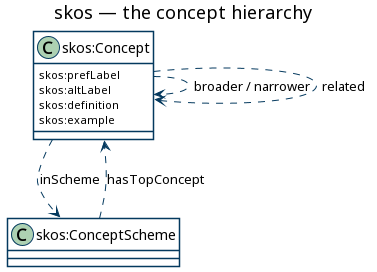
\includegraphics[width=\linewidth, height=0.6\textheight, keepaspectratio]{slides/im-101/skos/figs/skos.png}
    \end{column}
    \begin{column}{0.42\textwidth}
      \scriptsize
      \setlength{\itemsep}{0.5pt}
      \setlength{\parskip}{0pt}
      \textbf{Concepts}
      \begin{itemize}
        \item \texttt{skos:Concept} — a single idea in a vocabulary
        \item \texttt{skos:ConceptScheme} — the set that groups them
      \end{itemize}
      \vspace{0.4pt}
      \textbf{Relations (concept $\to$ concept)}
      \begin{itemize}
        \item \texttt{broader}\,$/\,$\texttt{narrower} — inverse hierarchy pair
        \item \texttt{related} — associative, non-hierarchical
        \item plus transitive variants (\ldots\texttt{Transitive})
      \end{itemize}
      \vspace{0.4pt}
      \textbf{Attributes \& membership}
      \begin{itemize}
        \item \texttt{prefLabel} / \texttt{altLabel} — display terms
        \item \texttt{definition} / \texttt{example} — meaning
        \item \texttt{inScheme} / \texttt{hasTopConcept}
      \end{itemize}
      \vspace{2pt}
      \begin{alertblock}{}
        A vocabulary is not an \emph{information model} — it is the \textbf{L0}
        layer: the named concepts we \emph{reuse} to describe L1.
      \end{alertblock}
    \end{column}
  \end{columns}
\end{frame}

\begin{frame}{RDFS / OWL — the vocabulary model (L1)}
  \framesubtitle{Classes, properties, and how they relate}

  \begin{columns}[T]
    \begin{column}{0.56\textwidth}
      \centering
      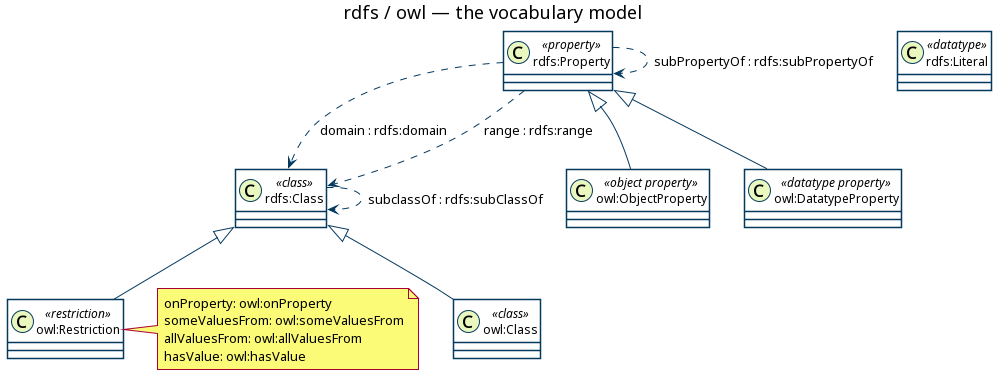
\includegraphics[width=\linewidth, height=0.6\textheight, keepaspectratio]{slides/im-101/rdfs-owl/figs/rdfs-owl.png}
    \end{column}
    \begin{column}{0.42\textwidth}
      \scriptsize
      \setlength{\itemsep}{0.5pt}
      \setlength{\parskip}{0pt}
      \textbf{Classes}
      \begin{itemize}
        \item \texttt{rdfs:Class}, \texttt{owl:Class} — \emph{sets} of resources
        \item \texttt{owl:Restriction} — anonymous classes
      \end{itemize}
      \vspace{0.4pt}
      \textbf{Properties}
      \begin{itemize}
        \item \texttt{owl:ObjectProperty} — links to a \emph{resource}
        \item \texttt{owl:DatatypeProperty} — links to a \emph{literal}
      \end{itemize}
      \vspace{0.4pt}
      \textbf{The glue}
      \begin{itemize}
        \item \texttt{rdfs:subClassOf} / \texttt{rdfs:subPropertyOf}
        \item \texttt{rdfs:domain} / \texttt{rdfs:range}
      \end{itemize}
      \vspace{2pt}
      \begin{alertblock}{}
        Open world: nothing is \emph{forbidden} unless you say so.
      \end{alertblock}
    \end{column}
  \end{columns}
\end{frame}

\begin{frame}{SHACL — the constraint model (L2)}
  \framesubtitle{Shapes: what a valid instance must look like}

  \begin{columns}[T]
    \begin{column}{0.56\textwidth}
      \centering
      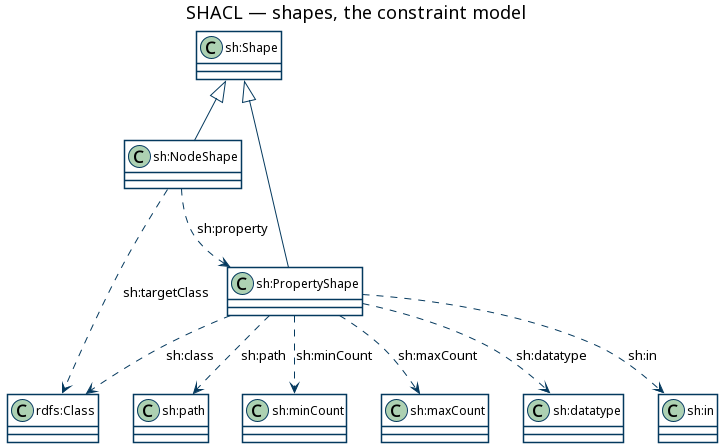
\includegraphics[width=\linewidth, height=0.6\textheight, keepaspectratio]{slides/im-101/shacl/figs/shacl.png}
    \end{column}
    \begin{column}{0.42\textwidth}
      \scriptsize
      \setlength{\itemsep}{0.5pt}
      \setlength{\parskip}{0pt}
      \textbf{Shapes}
      \begin{itemize}
        \item \texttt{sh:NodeShape} — constraints on a \emph{whole node}
        \item \texttt{sh:PropertyShape} — constraints on \emph{one property}
      \end{itemize}
      \vspace{0.4pt}
      \textbf{Targeting}
      \begin{itemize}
        \item \texttt{sh:targetClass} — which class the shape applies to
      \end{itemize}
      \vspace{0.4pt}
      \textbf{Property-shape constraints}
      \begin{itemize}
        \item \texttt{sh:in} — a closed value set
        \item \texttt{sh:datatype} — the value type
        \item \texttt{sh:minCount} / \texttt{sh:maxCount} — cardinality
        \item \texttt{sh:path} — which property
      \end{itemize}
      \vspace{2pt}
      \begin{alertblock}{}
        Closed world: what is missing \emph{means} something here.
      \end{alertblock}
    \end{column}
  \end{columns}
\end{frame}


\section{What it means to define an information standard}
\subsection{Challenges for integrating information standards}
\begin{frame}{Challenges for integrating information standards}

    \begin{itemize}
        \item Information standards are modelled according to different conventions
        \begin{itemize}
            \item CIM, INSPIRE $\rightarrow$ UML
            \item openADR (OpenAPI) $\rightarrow$ OpenAPI
            \item prov-o $\rightarrow$  OWL
        \end{itemize}
        \pause
        \item Information standards use different terms to define the same concept
        \item Information standards use the same terms to mean different things
        \pause
        \item Information standards are defined from the perspective of a specific domain and are not equally specific about every concept
        \begin{itemize}
            %\item CIM cares a lot about PowerSystemResources
            \item CIM doesn't think of Addresses as identifiable objects
            \item INSPIRE thinks of a Substation primarily as a point on a map (it models it as an `Appurtenance', as it does switches, transformers etc), you have to look in the AppurtenanceType enumeration to figure out what the object represents
            \item INSPIRE makes no distinction between Asset and PowerSystemResources
        \end{itemize}
    \end{itemize}
    
\end{frame}
\subsection{Proposed requirements}
\begin{frame}{What a well-defined information standard should be able to do}
    %\framesubtitle{Motivating the upcoming topics}

    \begin{requirement}\label{req:universal}
        An information standard must serve multiple use cases
    \end{requirement}

    \pause

    \begin{requirement}\label{req:technology}
        An information standard must not favor specific implementation technologies
    \end{requirement}

    \pause

    \begin{requirement}\label{req:consistent}
        An information standard must not contain logical inconsistencies (definitions of empty sets)
    \end{requirement}
\end{frame}

\subsection{Roadmap}
\begin{frame}{Roadmap: how the rest of today addresses the requirements}
  \framesubtitle{One requirement at a time — then an \textit{in practice} act applying them all}

  \setlength{\tabcolsep}{5pt}
  \renewcommand{\arraystretch}{1.3}
  \begin{center}
    \footnotesize
    \begin{tabular}{@{}p{4.8cm}p{7.0cm}@{}}
      \toprule
      \textbf{Requirement} & \textbf{Addressed by}\\
      \midrule
      \textbf{Req. \ref{req:universal}} --- serve multiple use cases &
        Kinds of information models: separating \emph{vocabulary} from \emph{constraint};
        later: profiles as use-case-specific L2 models\\
      \textbf{Req. \ref{req:technology}} --- technology-agnostic &
        MOF: metamodels, expressivity, choosing a \emph{pivot model},
        metamodel transformations; later: generated artifacts (Avro, JSON Schema, SQL)\\
      \textbf{Req. \ref{req:consistent}} --- no logical inconsistencies &
        Upper ontologies \& ontology alignment: spotting and fixing semantic conflicts (the
        \texttt{cim:Outage} example)\\
      \bottomrule
    \end{tabular}
  \end{center}

  \vspace{0.1cm}
  \begin{block}{The goal}
    A practical guide to how to meet all these requirements. Looking at how Netbeheer Nederland addresses them. And finally looking back at openADR.
  \end{block}
\end{frame}


\section{Requirement 1: kinds of information models}
\begin{frame}
  \epigraph{\huge Requirement 1: serving multiple use cases}{An information standard must serve multiple use cases}
\end{frame}

\subsection{Kinds of Models}\label{subsec:KindsofModels}


\begin{frame}{Kinds of Models}    \framesubtitle{Natural and formal languages}


    \AddToShipoutPictureFG*{
        \AtPageUpperLeft{\put(-5,-15){\makebox[\paperwidth][r]{Requirement 1}}}  
        }%


\begin{onlyenv}<1>
    \begin{center}
\begin{figure}
    \centering
    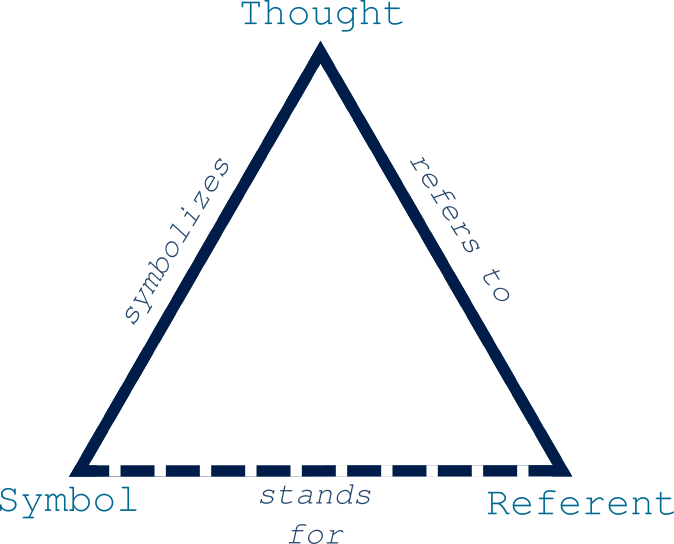
\includegraphics[height =0.5 \textheight, keepaspectratio]{slides/kinds/semantic-triangle/figs/SemanticTriangle.png}
    \caption{Semantic Triangle}
    \label{fig:SemanticTriangle}
\end{figure}
\end{center}
\end{onlyenv}

\begin{onlyenv}<2>
    \begin{center}
\begin{figure}
    \centering
    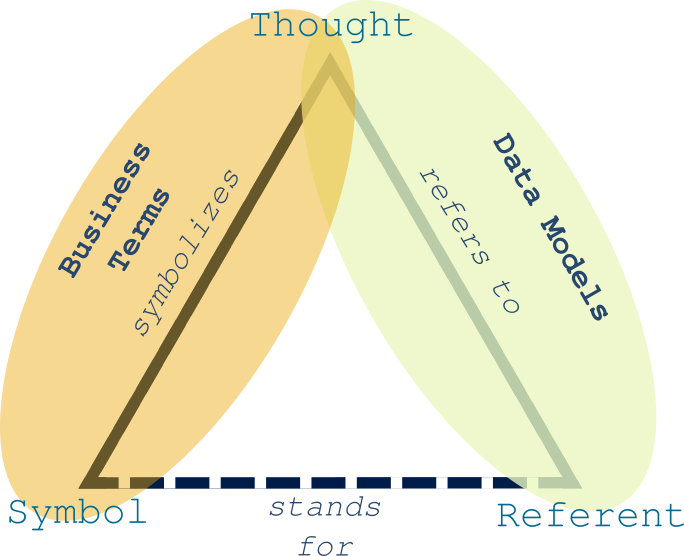
\includegraphics[height =0.5 \textheight, keepaspectratio]{slides/kinds/semantic-triangle/figs/SemanticTriangleModels.png}
    \caption{Semantic Triangle}
    
\end{figure}
\end{center}
\end{onlyenv}
  
\end{frame}
\subsection{Kinds of Models}
\begin{frame}{Kinds of Models}
    \framesubtitle{Vocabularies and Constraints}


    \AddToShipoutPictureFG*{
    \AtPageUpperLeft{\put(-5,-15){\makebox[\paperwidth][r]{Requirement 1}}}
    }%

        \begin{table}[]
            \begin{tabular}{ccc}
                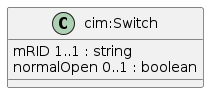
\includegraphics[width=0.3\textwidth]{slides/kinds/switches-examples/figs/switch1.png}& 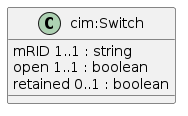
\includegraphics[width=0.3\textwidth]{slides/kinds/switches-examples/figs/switch2.png} & 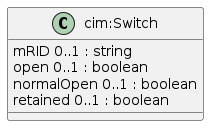
\includegraphics[width=0.3\textwidth]{slides/kinds/switches-examples/figs/SwitchVocab.png} \\
            \multicolumn{1}{l}{}                                                        & \multicolumn{1}{l}{}                                                                 & \multicolumn{1}{l}{}                                                          \\
            \begin{tabular}[c]{@{}c@{}}a Switch class with \\ 2 attributes\end{tabular} & \begin{tabular}[c]{@{}c@{}}a Switch class with\\ 2 different attributes\end{tabular} & \begin{tabular}[c]{@{}c@{}}a Switch class with \\ all attributes\end{tabular} \\
            some compulsory                                                             & some compulsory                                                                      & all optional                                                                
            \end{tabular}
        \end{table}
\end{frame}

\begin{frame}{Kinds of Models}
    \framesubtitle{Vocabularies and constraints, definitions}

    \AddToShipoutPictureFG*{
    \AtPageUpperLeft{\put(-5,-15){\makebox[\paperwidth][r]{Requirement 1}}}
    }%

   \begin{definition}
   \colorbox{newlightblue}{Vocabulary Model}: Models the reusable terms of the things the model describes using the open world assumption. This is the part of an information model that is reusable across use cases
   \end{definition}

   \begin{definition}
   \colorbox{neworange}{Constraint Model}: Models the data structure of the things the model describes using the closed world assumption. This part of an information model is use case specific
   \end{definition}
\end{frame}

\begin{frame}{Kinds Of Models}
    \framesubtitle{A rough taxonomy of models}


    \AddToShipoutPictureFG*{
    \AtPageUpperLeft{\put(-5,-15){\makebox[\paperwidth][r]{Requirement 1}}}
    }%


    \begin{figure}
        \centering
        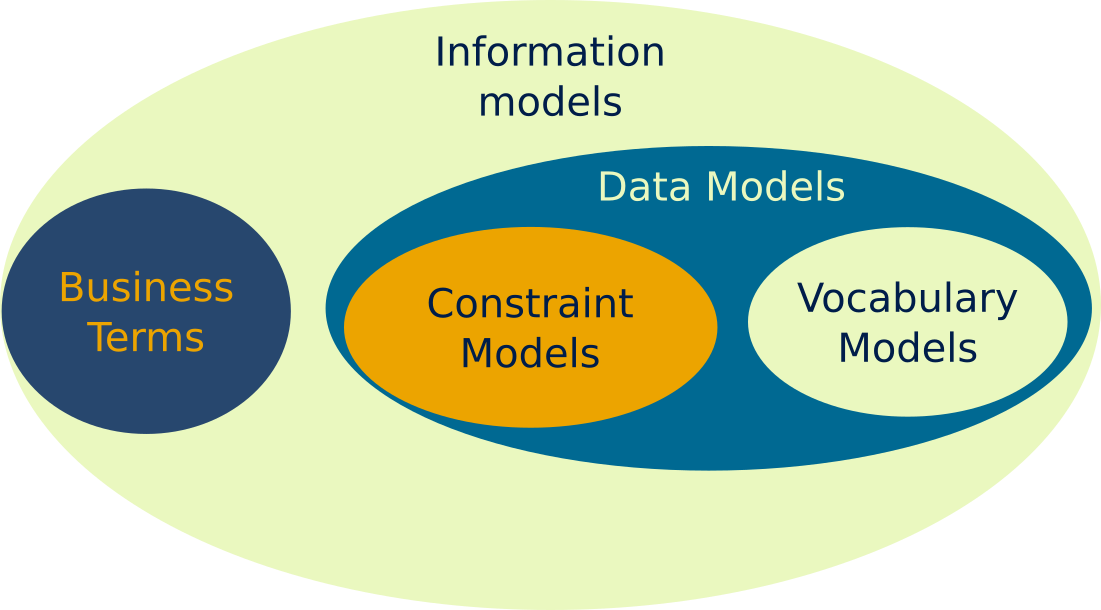
\includegraphics[height =0.55 \textheight, keepaspectratio]{slides/kinds/model-taxonomy/figs/ModelTaxonomy.png}
        \caption{Venn diagram of model types}
        \label{fig:ModelTaxonomy}
    \end{figure}
\end{frame}

\AddToShipoutPictureFG*{
    \AtPageUpperLeft{\put(-5,-15){\makebox[\paperwidth][r]{Requirement 1}}}
    }%

\begin{frame}{Addressing requirement \ref{req:universal}}
    \begin{itemize}
        \item An information standard must serve multiple use cases (Req. \ref{req:universal}), which requires:
        \begin{itemize}
            \item Separation of vocabulary and constraint models
            \item Focussing on vocabulary model integration
            \item Using the Open World Assumption for vocabulary integration
        \end{itemize}
    \end{itemize}
\end{frame}


\section{Requirement 2: MOF, expressivity, and transformation}
\begin{frame}
  \epigraph{\huge Requirement 2: being information technology-agnostic}{An information standard must not favor specific implementation technologies}
\end{frame}

\begin{frame}{Models of Models}\subsection{Models of Models}


    \AddToShipoutPictureFG*{
        \AtPageUpperLeft{\put(-5,-15){\makebox[\paperwidth][r]{Requirement 2}}}  
        }%


\begin{table}[]
\begin{tabular}{l|cc}
\textbf{meta-meta-models} & \multicolumn{2}{c}{MOF, RDF(S)}                                                                                                                                                                                              \\ \hline
\textbf{meta-models}      & \multicolumn{2}{c}{\begin{tabular}[c]{@{}c@{}}UML, RDFS/OWL, SHACL, SQL, \\ JSON-schema, Avro Schema,XSD, ecore\end{tabular}}                                                                                             \\ \hline
\textbf{models}           & \multicolumn{1}{c|}{\cellcolor{newlightblue}\begin{tabular}[c]{@{}c@{}}IEC-CIM, 61850, HR-XML, \\ prov-o, ssn, qudt, dcat\\dqv, INSPIRE, nen-2660,\\ BFO, IFC...\end{tabular}} & \cellcolor{neworange}\begin{tabular}[c]{@{}c@{}}CIM-EQ, CIM-SSH, \\ CIM-SV, DCAT-AP, GML...\end{tabular} \\ \hline
\textbf{instance data}    & \multicolumn{2}{c}{substations, employees, events, meters etc.}                                                                                                                                                          
\end{tabular}
\end{table}                                                                         
\end{frame}
\begin{frame}{Meta-model Expressivity}
    \subsection{Meta-model Expressivity}\label{subsec:MetaModelExpressivity}
    

    \AddToShipoutPictureFG*{
        \AtPageUpperLeft{\put(-5,-15){\makebox[\paperwidth][r]{Requirement 2}}}  
        }%

    
    \begin{table}[]
        \resizebox{\textheight}{!}{
        \begin{tabular}{lcr}
        \textbf{Construct}  & \textbf{Description}                                                                     \\ \hline%& \textbf{\begin{tabular}[c]{@{}r@{}}Description Logic \\ expressivity\end{tabular}} \\ \hline
        data structure      & how data about a thing is structured                                                     \\ \hline%& \\ \hline
        set (class)         & a set of things                                                                          \\ \hline%&    $\mathcal{A}\mathcal{L}$                                                                             \\ \hline
        individual          & a single thing                                                                           \\ \hline%&                                                                                    \\ \hline
        role                & \begin{tabular}[c]{@{}c@{}}properties, attributes,\\ relationships\end{tabular}          \\ \hline%&                                                                                    \\ \hline
        datatype            & ways to format literals                                                                  \\ \hline%&                                                                                    \\ \hline
        set membership      & \begin{tabular}[c]{@{}c@{}}ability to say an individual \\ belongs to a set\end{tabular} \\ \hline%&                                                                                    \\ \hline
        set inclusion       & \begin{tabular}[c]{@{}c@{}}subclass/superclass \\ relationships\end{tabular}             \\ \hline%&                                                                                    \\ \hline
        set equivalence     & \begin{tabular}[c]{@{}c@{}}ability to say 2 sets are\\  actually the same\end{tabular}   \\ \hline%&                                                                                    \\ \hline
        set disjunctiveness & \begin{tabular}[c]{@{}c@{}}ability to say 2 sets \\ share no individuals\end{tabular}    \\ \hline%&                                                                                   \\ \hline
        cardinality restrictions & \begin{tabular}[c]{@{}c@{}}ability to say how often \\ a role may occur\end{tabular}          \\ \hline%& 
        
        \end{tabular}}
        \end{table}
\end{frame}
\begin{frame}{Comparing expressivity}

    \AddToShipoutPictureFG*{
        \AtPageUpperLeft{\put(-5,-15){\makebox[\paperwidth][r]{Requirement 2}}}  
        }%
 
\begin{table}
    \resizebox{\textwidth}{!}{
    \begin{tabular}{lcccccccc}
        & \multicolumn{1}{l|}{Open World Assumption}                                                     & \multicolumn{2}{l}{Closed World Assumption}  \\\cline{2-8}
    \textbf{Construct}       & \textbf{RDFS/OWL}    & \textbf{SHACL} & \textbf{LinkML}   & \textbf{UML}       & \textbf{\begin{tabular}[c]{@{}c@{}}JSON \\ Schema**\end{tabular}} & \textbf{\begin{tabular}[c]{@{}c@{}}Apache \\ Avro\end{tabular}}   & \textbf{SQL}       & \textbf{XSD}          \\ \hline
    data structure           & \multicolumn{1}{l}{} & x              & x                 & \multirow{2}{*}{x} & \multirow{2}{*}{x}                                                & \multirow{2}{*}{x}                                                & \multirow{2}{*}{x} & \multirow{2}{*}{x}    \\ \cline{1-4}
    set (class)              & x                    &                & kinda...          &                    &                                                                   &                                                                   &                    &                       \\ \hline
    individual               & x                    & x              & x                 & x                  & x                                                                 & x                                                                 & x                  & x                     \\ \hline
    role                     & x                    & x              & x                 & x                  & x                                                                 & x                                                                 & x                  & x                     \\ \hline
    datatype                 & x                    & x              & x                 & x                  & x                                                                 & x                                                                 & x                  & x                     \\ \hline
    set membership           & x                    &                &                   & x                  &                                                                   &                                                                   & x                  & x                     \\ \hline
    set inclusion            & x                    & kinda...       & kinda...          & kinda...           & kinda...                                                          &                                                                   & x                  & kinda...              \\ \hline
    set equivalence          & x                    &                &                   &                    &                                                                   &                                                                   &                    &                       \\ \hline
    set disjunctiveness      & x                    &                &                   & implied            & implied                                                           & implied                                                           & implied            & implied               \\ \hline
    cardinality restrictions & x                    & x              & x                 & x                  & x                                                                 & limited                                                           & limited            & x                    
    \end{tabular}
    }
    %\caption{ *:open world assumption applies, **: closed world assumption applies}
\end{table}
    

    
\end{frame}
\subsection{Towards technology-agnostic information standards}
\begin{frame}{Towards technology-agnostic information standards}
\framesubtitle{Choosing a pivot model}

\AddToShipoutPictureFG*{
    \AtPageUpperLeft{\put(-5,-15){\makebox[\paperwidth][r]{Requirement 2}}}  
    }%
 
\begin{table}[overview of supported constructs for different meta-models]
    \resizebox{\textwidth}{!}{
    \begin{tabular}{lacoccccc}
        & \multicolumn{1}{l|}{Open World Assumption}                                                     & \multicolumn{2}{l}{Closed World Assumption}  \\\cline{2-8}
    \textbf{Construct}       & \textbf{RDFS/OWL}    & \textbf{SHACL}         & \textbf{LinkML}  & \textbf{UML}     & \textbf{\begin{tabular}[c]{@{}c@{}}JSON \\ Schema\end{tabular}} & \textbf{\begin{tabular}[c]{@{}c@{}}Apache \\ Avro\end{tabular}} & \textbf{SQL}     & \textbf{XSD}     \\ \hline
    data structure           &                      & x                      & x                & \multirow{2}{*}{x}                & \multirow{2}{*}{x}                                                & \multirow{2}{*}{x}                                                & \multirow{2}{*}{x} & \multirow{2}{*}{x} \\ \cline{1-4}
    set (class)              & x                    &                        & kinda...         &                    &                                                                   &                                                                   &                    &                    \\ \hline
    individual               & x                    & x                      & x                & x                  & x                                                                 & x                                                                 & x                  & x                  \\ \hline
    role                     & x                    & x                      & x                & x                  & x                                                                 & x                                                                 & x                  & x                  \\ \hline
    datatype                 & x                    & x                      & x                & x                  & x                                                                 & x                                                                 & x                  & x                  \\ \hline
    set membership           & x                    &                        &                  & x                  &                                                                   &                                                                   & x                  & x                  \\ \hline
    set inclusion            & x                    & kinda...               & kinda...         & kinda...           & kinda...                                                          &                                                                   & x                  & kinda...           \\ \hline
    set equivalence          & x                    &                        &                  &                    &                                                                   &                                                                   &                    &                    \\ \hline
    set disjunctiveness      & x                    &                        &                  & implied            & implied                                                           & implied                                                           & implied            & implied            \\ \hline
    cardinality restrictions & x                    & x                      & x                & x                  & x                                                                 & limited                                                           & limited            & x                 
    \end{tabular}
    }
    %\caption{Open world and high expressivity for vocabulary model, distinct constructs for constraint model}
\end{table}
    

    
\end{frame}
\begin{frame}{Towards technology-agnostic information standards}
    \framesubtitle{Meta-model transformations}
    
    \AddToShipoutPictureFG*{
        \AtPageUpperLeft{\put(-5,-15){\makebox[\paperwidth][r]{Requirement 2}}}  
        }%  

    \begin{table}[overview of supported constructs for different meta-models]
        \resizebox{\textwidth}{!}{
        \begin{tabular}{lccccccccc}
            & \multicolumn{1}{l|}{Open World Assumption}                                                     & \multicolumn{2}{l}{Closed World Assumption}  \\\cline{2-8}
        \textbf{Construct}       & \textbf{RDFS/OWL}        & \textbf{SHACL}                      & \textbf{LinkML}                          & \textbf{UML(xmi)}                & \textbf{\begin{tabular}[c]{@{}c@{}}JSON \\ Schema\end{tabular}} & \textbf{\begin{tabular}[c]{@{}c@{}}Apache \\ Avro\end{tabular}}     & \textbf{SQL}               & \textbf{XSD}     \\ \hline
        data structure           & \multicolumn{1}{l}{}     & \tiny{Class}                        & \tiny{Class}                             & \multirow{2}{*}{\tiny{Class}} & \multirow{2}{*}{\tiny{object}}                                    & \multirow{2}{*}{\tiny{record}}                                        & \multirow{2}{*}{\tiny{table}}     & \multirow{2}{*}{\tiny{complexType}} \\ \cline{1-3}
        set (class)              & \tiny{Class}             &                                     & \tiny{class\_uri}                        &                               &                                                                   &                                                                       &                                   &                    \\ \hline
        individual               & \tiny{Resource}          & \tiny{Resource}                     & \tiny{permissible\_values}               & \tiny{Instance}               & \tiny{instance}                                                   & implied                                                               & \tiny{record}                     & \tiny{complex element}                  \\ \hline
        role                     & \tiny{Property}          & \tiny{PropertyShape}                & \tiny{Slot}                              & \tiny{Property}               & \tiny{property}                                                   & \tiny{field}                                                          & \tiny{column}                     & \tiny{attribute}                  \\ \hline
        datatype                 & \tiny{DataType}          & \tiny{DatatypeConstraintComponent}  & \tiny{Type}                              & \tiny{Primitve}               & \tiny{basic type}                                                 & \tiny{Primitive Type}                                                 & \tiny{data type}                  & \tiny{Datatype}    \\ \hline
        set membership           & \tiny{type}              &                                     &                                          & \tiny{type}                   &                                                                   &                                                                       & implied                           & implied                  \\ \hline
        set inclusion            & \tiny{subClassOf}        & \tiny{and***}                       & \tiny{is\_a}                             & \tiny{Generalization***}      & \tiny{allOf***}                                                   &                                                                       & \tiny{union}                      & \tiny{extension***}           \\ \hline
        set equivalence          & \tiny{EquivalentClass}   &                                     &                                          &                               &                                                                   &                                                                       &                                   &                    \\ \hline
        set disjunctiveness      & \tiny{disjointWith}      &                                     &                                          & implied                       & implied                                                           & implied                                                               & implied                           & implied            \\ \hline
        cardinality restrictions & \tiny{min/maxCardinality}& \tiny{min/maxCount}                 & \tiny{minimum/maximum\_cardinality}      & \tiny{lower/upperValue}       & \tiny{min/maxItems}                                               & limited                                                               & limited                           & \tiny{min/maxOccurs}                 
        \end{tabular}
        }
        %\caption{ *:open world assumption applies, **: closed world assumption applies,***: more of a part-whole relationship at data structure level}
        \end{table}
\end{frame}




\begin{frame}{Addressing requirement \ref{req:technology}}
    \begin{itemize}
        \item An information standard must not favor specific implementation technologies (Req. \ref{req:technology}), which requires:
        \begin{itemize}
            \item An understanding of models, meta-models, and in some cases meta-meta-models
            \item The ability to transform both vocabulary models as well as constraint models between technologies (and their respective meta-models)
            \item The selection of a pivot model that has sufficient expressivity to allow transformation to all (most) other meta-models
        \end{itemize}
    \end{itemize}
\end{frame}

\section{Ontology, meaning, and the open world}
% \begin{frame}{Ontologies, meaning, and the open world assumption}

  \begin{itemize}
    \item A \textbf{vocabulary model} is a community agreement: \emph{what the sets contain}.
    \begin{itemize}
      \item \texttt{Terminal}, \texttt{ConnectivityNode}, \texttt{AnalogValue}, \texttt{PhaseCode} — reusable across use cases, across organizations.
    \end{itemize}
    \pause
    \item The \textbf{Open World Assumption (OWA)}:
    \begin{itemize}
      \item what data does \emph{not} say is \emph{not false} — someone else may say more
      \item different data can say \emph{more} about the same world without contradicting each other
      \item this is what makes \emph{integration} of different standards possible at all
    \end{itemize}
    \pause
    \item The \textbf{Closed World Assumption (CWA)} allows us to validate data against rules:
    \begin{itemize}
      \item a profile / schema says: \emph{this is what the data is supposed to look like}
      \item this is what makes \emph{validation} and \emph{interoperability of implementations} possible
    \end{itemize}
  \end{itemize}

\end{frame}

\begin{frame}{Some Definitions}

    \AddToShipoutPictureFG*{
        \AtPageUpperLeft{\put(-5,-15){\makebox[\paperwidth][r]{Requirement 1}}}  
        }%

    \begin{definition}
        Closed World Assumption (CWA): \textit{Information that is unknown is presumed to be false} 
    \end{definition}

    \begin{definition}
        Open World Assumption(OWA): \textit{Information that is unknown is presumed neither true nor false}
    \end{definition}

    \begin{definition}
        Unique Naming Assumption(UNA): \textit{Different names are presumed to refer to different things in reality (this is a specific consequence of the CWA)}
    \end{definition}
        
    
\end{frame}
\begin{frame}{Avoiding Inconsistencies}
    \subsection{Handling Inconsistencies}
\framesubtitle{Some definitions}
    \footnotesize

\AddToShipoutPictureFG*{
    \AtPageUpperLeft{\put(-5,-15){\makebox[\paperwidth][r]{Requirement 3}}}
    }%

    \begin{definition}
        Universe of Discourse: \textit{The set of entities over which certain variables of interest in some formal treatment may range}
    \end{definition}

    \begin{definition}
        Modelling adequacy: \textit{The degree to which a model is capable of describing relevant phenomena. The accuracy with which the variables in the model describe the entities in the real world}
    \end{definition}

    \begin{definition}
        Interpretation: \textit{An assignment of meaning to the symbols of a formal language}
    \end{definition}


    \begin{definition}
        Interpreter's expectation of a model: \textit{The variables that an interpreter (domain expert) expects to be in the Universe of Discourse}
    \end{definition}
\end{frame}


\section{Requirement 3: ontology alignment and upper ontologies}
\begin{frame}
  \epigraph{\huge Requirement 3: being consistent}{An information standard must not contain logical inconsistencies (definitions of empty sets)}
\end{frame}

\begin{frame}{Avoiding Inconsistencies}
    \framesubtitle{Example}

    \AddToShipoutPictureFG*{
    \AtPageUpperLeft{\put(-5,-15){\makebox[\paperwidth][r]{Requirement 3}}}
    }%


        \begin{figure}
            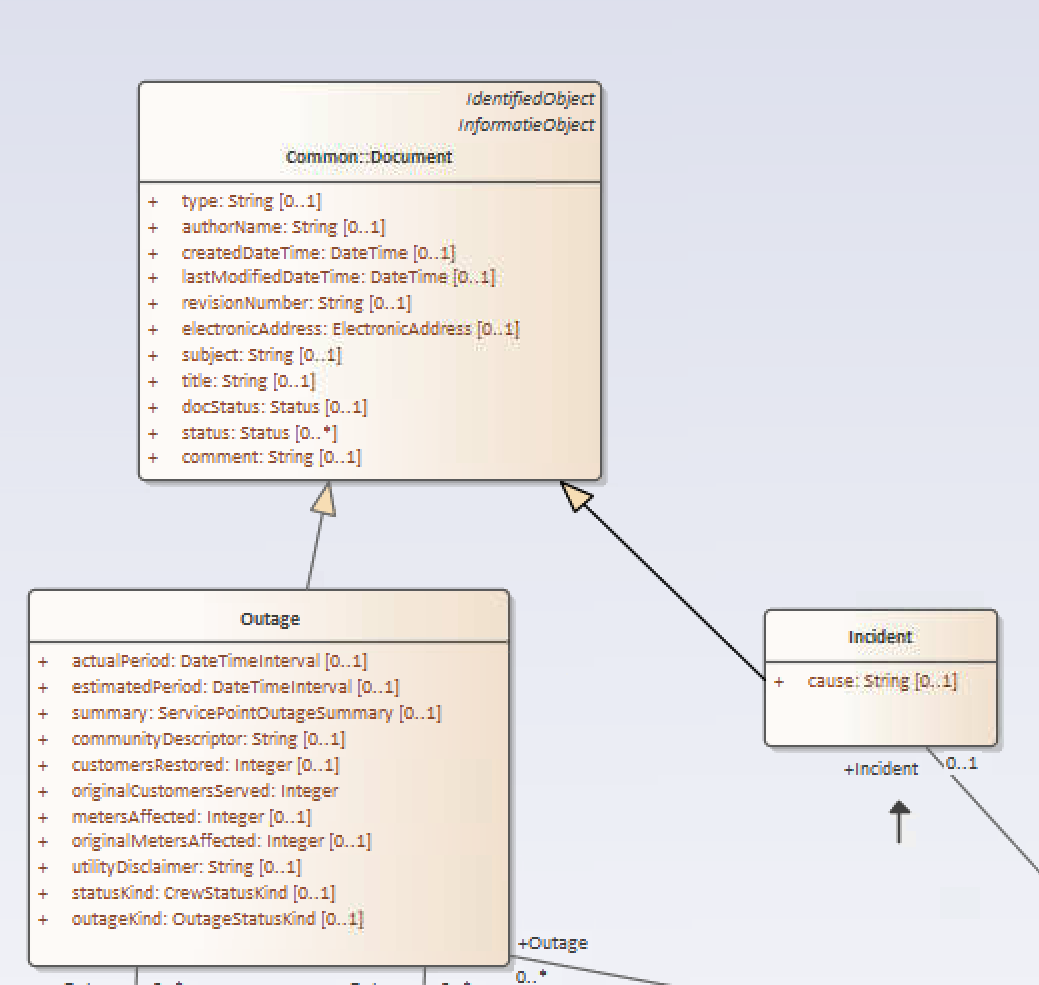
\includegraphics[height=0.6\textheight, keepaspectratio]{slides/alignment/outage-example/figs/outage.png}
            \caption{Events or States modelled as Documents}
        \end{figure}


\end{frame}

\subsection{Upper Ontologies}
\begin{frame}{Using Upper Ontologies}
    \framesubtitle{Intro and benefits}

    \AddToShipoutPictureFG*{
    \AtPageUpperLeft{\put(-5,-15){\makebox[\paperwidth][r]{Requirement 3}}}
    }%

    \begin{itemize}
        \item Upper ontologies provide a high over classification framework that can form the basis for interpreting models describing different Universes of Discourse
        \item Upper ontologies can make integrating information standards a lot easier and more formal
        \item Upper ontologies make basic assumptions about our reality explicit
        \item Two relevant examples
        \begin{itemize}
            \item Basic Formal Ontology (BFO): well known in the scientific Linked Data community
            \item nen-2660: the Upper Ontology for the Dutch construction industry. A simplified version of the BFO
        \end{itemize}
    \end{itemize}
\end{frame}

\begin{frame}{Using Upper Ontologies}
    \framesubtitle{Limitations and pitfalls}

    \AddToShipoutPictureFG*{
    \AtPageUpperLeft{\put(-5,-15){\makebox[\paperwidth][r]{Requirement 3}}}
    }%

    \begin{itemize}
        \item Upper ontologies enforce a specific perspective on the world
        \begin{itemize}
            \item This creates barriers for underrepresented perspectives of what, for example, the energy system 'is' and what its existence (or lack thereof) implies for people or other things with intrinsic value, and representing those perspectives in data
            \item This could be a criticism of any applied formal language (and therefore all structured data)
        \end{itemize}
        \pause
        \item Upper ontologies can get very intangible, causing domain experts to be unable to validate a model
        \begin{itemize}
            \item Explain to an asset manager that their inspection report is actually also a "generically dependent continuant" (BFO)...
            %\item I consider myself reasonably knowledgeable about this subject but I'm not sure this is a correct example
        \end{itemize}
        \pause
        \item Upper ontologies are often less formal than they seem to suggest
        \begin{itemize}
            \item nen-2660 considers an Organization to be a Physical Object
            \item I'm still on the fence whether an 'upper ontology' is the way to go, or if 'upper business terms' are a more accurate representation
        \end{itemize}
    \end{itemize}
\end{frame}

\begin{frame}{Using Upper Ontologies}
    \framesubtitle{Example (my personal favorite)}

    \AddToShipoutPictureFG*{
    \AtPageUpperLeft{\put(-5,-15){\makebox[\paperwidth][r]{Requirement 3}}}
    }%

    \begin{figure}
        \centering
        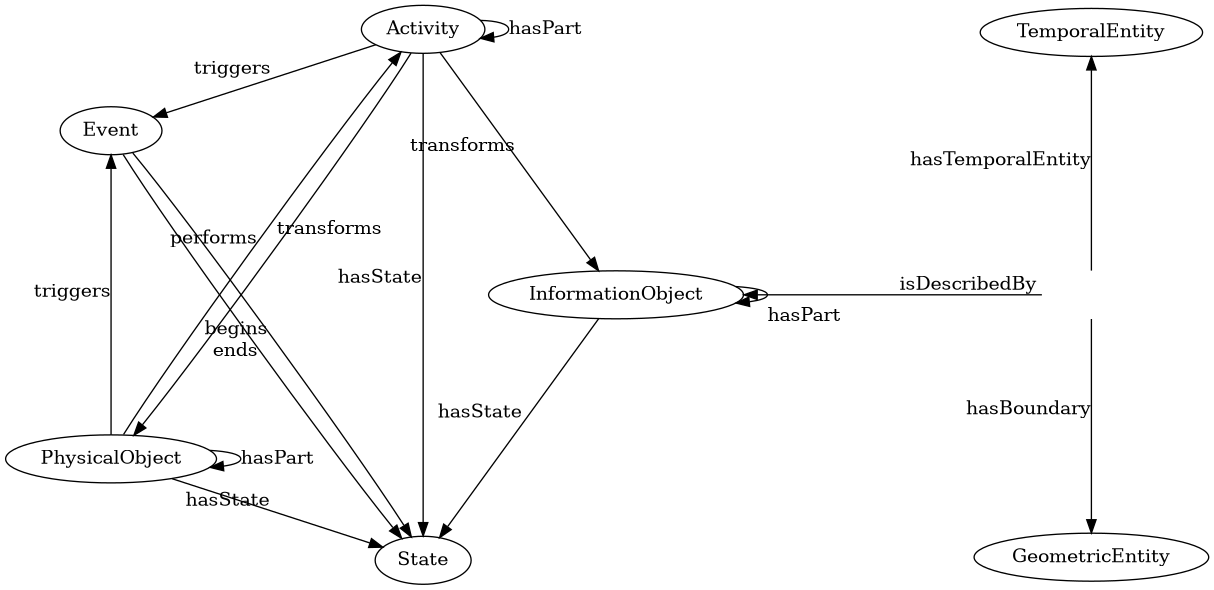
\includegraphics[height= 0.55 \textheight, keepaspectratio]{slides/alignment/upper-ontologies-example/figs/UpperOntology.png}
        \caption{Upper ontology suggested by nen-2660}
        \label{fig:UpperOntology}
    \end{figure}
\end{frame}

\begin{frame}{Using upper ontologies}{Fixing a cim:Outage (according to nen-2660) }

    \AddToShipoutPictureFG*{
    \AtPageUpperLeft{\put(-5,-15){\makebox[\paperwidth][r]{Requirement 3}}}
    }%

    \begin{columns}[T] % align columns
        \begin{column}{.48\textwidth}
        \begin{figure}
            \centering
            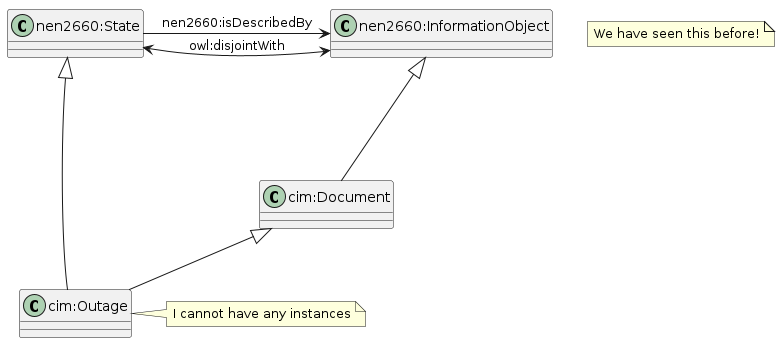
\includegraphics[width=1\textwidth]{slides/alignment/fixing-cim-outage/figs/AutageNaiveAttempt.png}
            \caption{Outage as State \textit{and} InformationObject}
        \end{figure}
        \end{column}%

        \begin{column}{.48\textwidth}
            \begin{figure}
                \centering
                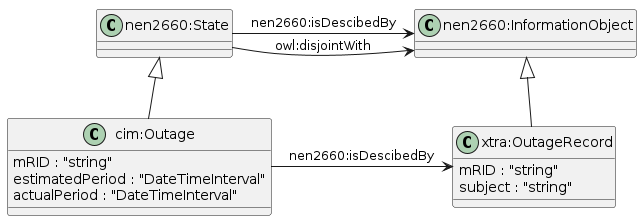
\includegraphics[width= 0.9 \textwidth]{slides/alignment/fixing-cim-outage/figs/FixingOutage.png}
                \caption{Separating the state from the record that describes it}
                \label{fig:FixingOutage}
            \end{figure}
        \end{column}
    \end{columns}
\end{frame}

% \include{slides/alignment/techniques}
\begin{frame}{Addressing requirement \ref{req:consistent}}
\begin{itemize} 
\item An information standard must not contain logical inconsistencies (definitions of empty sets) (Req. \ref{req:consistent}), which requires:
\begin{itemize}
    \item Semantic harmonization of the standards
    \item The selection of an upper ontology helps identify potential inconsistencies
\end{itemize}

\end{itemize}

\end{frame}

\section{In practice: one exchange, from the model (L1) to the artifacts (L3)}
\begin{frame}{A real example: LV measurement events}
	Low-voltage measurement values published on a Kafka topic.
	\vspace{0.4em}
	\begin{itemize}
		\item The current schema: an Avro file. 
		\item The same information is also stored in a warehouse (Postgres) and exposed via an HTTP query API
		\item Today these three exist side by side, maintained \emph{by hand}, and they occasionally disagree
	\end{itemize}
	\begin{block}{We will trace one event through L1, L2, L3}
	One event $\approx$ \emph{one sensor, one terminal, several measurements, several values}.
	\end{block}
\end{frame}

\begin{frame}{L1 — the measurement information model}
	\begin{columns}[T]
		\begin{column}{0.62\textwidth}
			\centering
			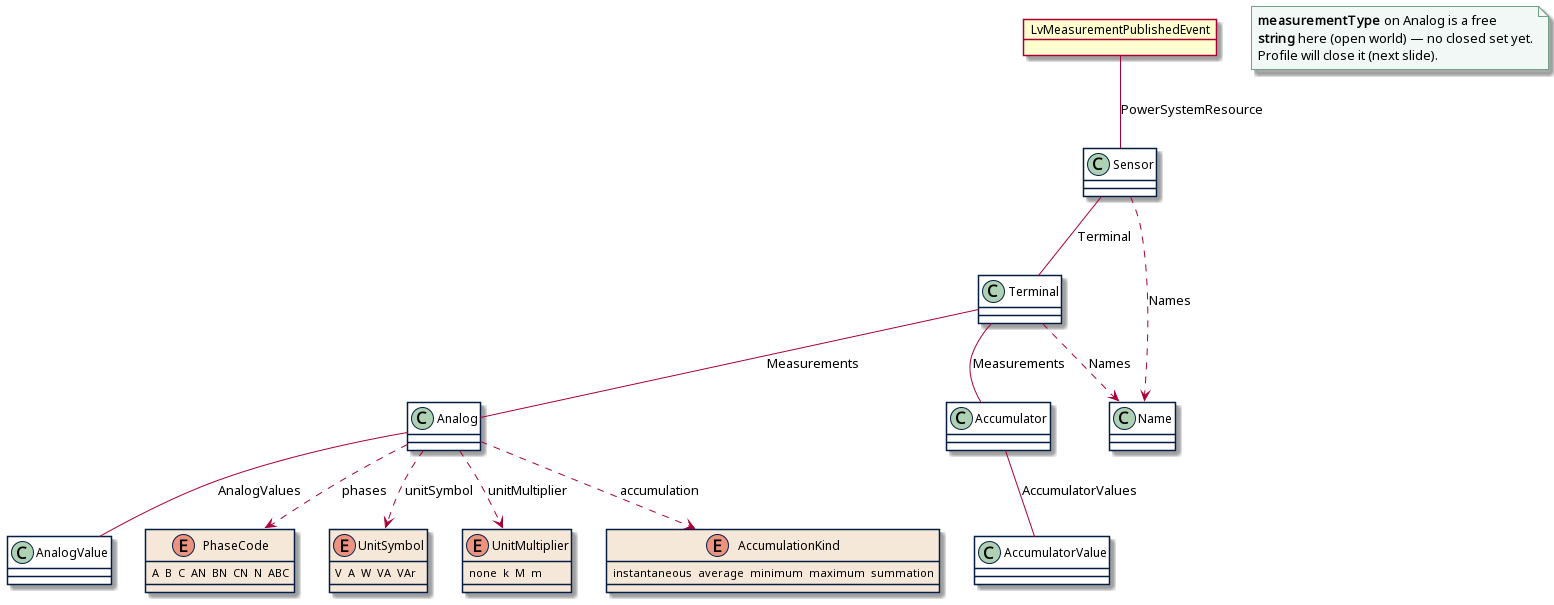
\includegraphics[width=\linewidth]{slides/exchange/example-information-model/figs/information-model.png}
		\end{column}
		\begin{column}{0.38\textwidth}
			\textbf{Everything here is standard or convention:}
			\begin{itemize}
				\scriptsize
				\item \texttt{Sensor, Terminal, Analog, Accumulator, AnalogValue} — CIM core classes (IEC 61970-301)
				\item \texttt{PhaseCode, UnitSymbol, UnitMultiplier} — CIM enumerations
				\item \texttt{mRID} — IEC 61970-552 identifier convention
				\item \texttt{QualityMetadata} — W3C DQV, re-used
			\end{itemize}
		\end{column}
	\end{columns}
	\vspace{0.3em}
	\alert{Nothing local, nothing proprietary.} This is what we get for free —
	the definitions our engineers currently re-type into every schema file.
\end{frame}

\begin{frame}{L2 — Profile (closed world)}
	\small
	A profile \emph{references} an information model and \emph{adds}:
	\begin{itemize}
		\item \textbf{scope constraints} — which parts of the Ontology are used
		\item \textbf{cardinalities} — required / optional / exactly-one
		\item \textbf{value-space} — closed enums, pattern, range

	\end{itemize}
	\vspace{0.4em}
	\begin{columns}[T]
		\begin{column}{0.5\textwidth}
			\begin{block}{Closed world}
				No statement is made if not in-scope. Absence \emph{means} something here.
			\end{block}
		\end{column}
		\begin{column}{0.5\textwidth}
			\begin{alertblock}{syntax agnostic}
				We are just describing what the data looks like, so it can be expressed in any syntax we might need, insuring consistent semantics across syntaxes.
			\end{alertblock}
		\end{column}
	\end{columns}
	
\end{frame}

\begin{frame}{L2 — the exchange profile}
	\begin{columns}[T]
		\begin{column}{0.55\textwidth}
			\centering
			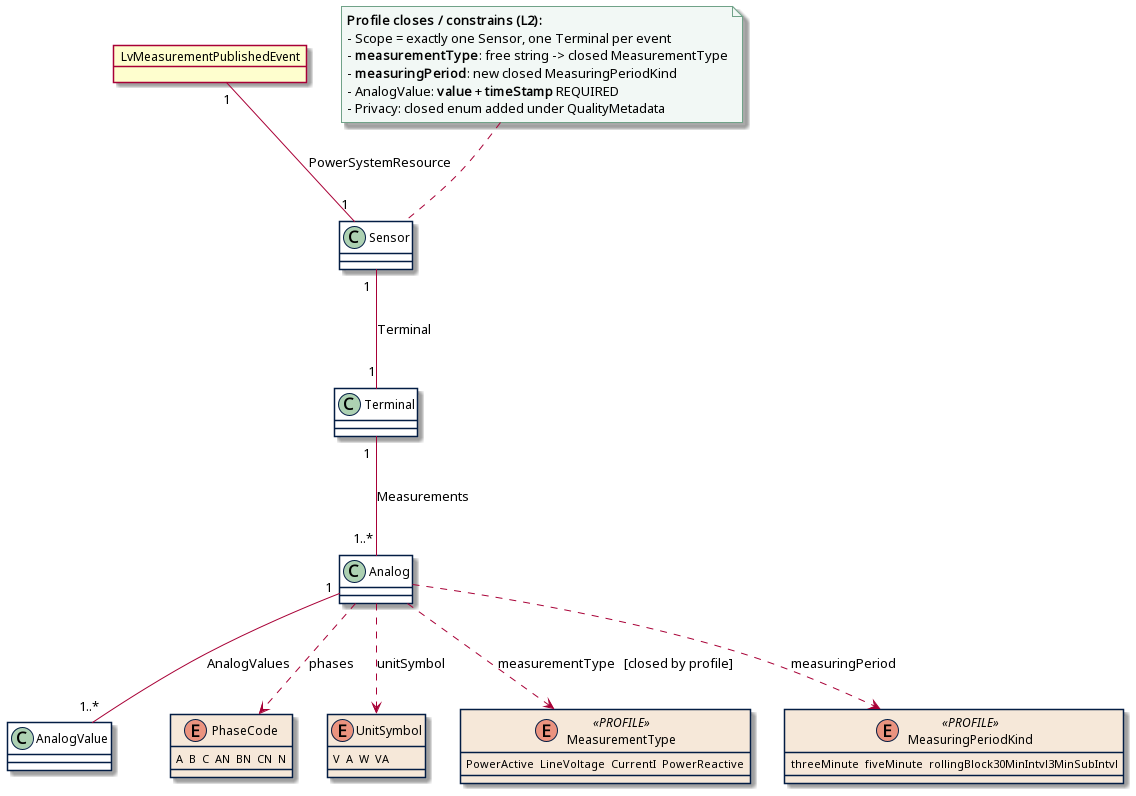
\includegraphics[width=\linewidth]{slides/profiles/example-profile/figs/profile.png}
		\end{column}
		\begin{column}{0.43\textwidth}
			\textbf{What the profile adds over the IM (constraints only):}
			\begin{itemize}
				\scriptsize
				\item two L1 enums \emph{closed} to the values of this exchange:
				  \texttt{MeasuringPeriodKind} and \texttt{Privacy}
				\item \texttt{measurementType} closed to: \texttt{PowerActive}, \texttt{LineVoltage}, \texttt{CurrentI}, \ldots
				\item required fields: every \texttt{AnalogValue} \emph{must} have \texttt{timeStamp} + \texttt{value}
				\item cardinalities: exactly one \texttt{Sensor}, one \texttt{Terminal} per event
			\end{itemize}
			\begin{block}{Still no format anywhere}
			\end{block}
		\end{column}
	\end{columns}
	\vspace{0.3em}
	This is the \emph{only} place those decisions are written down —
	not in three schema files, not in a wiki page.
\end{frame}

\begin{frame}{Artifact 1/3 — Avro (streaming, Kafka)}
	\begin{minipage}{0.98\linewidth}
	\lstinputlisting[style=code, basicstyle=\ttfamily\tiny, columns=fullflexible]{code/analog.avsc}
	\end{minipage}
\end{frame}

\begin{frame}{Artifact 2/3 — JSON Schema (request/response HTTP)}
	\begin{minipage}{0.98\linewidth}
	\lstinputlisting[style=code, basicstyle=\ttfamily\tiny, columns=fullflexible]{code/analog-measurement.json}
	\end{minipage}
\end{frame}

\begin{frame}{Artifact 3/3 — SQL DDL (batch / warehouse)}
	\begin{minipage}{0.99\linewidth}
	\lstinputlisting[style=code]{code/analog.sql}
	\end{minipage}
\end{frame}

\begin{frame}{Toolchain}
	\begin{columns}[T]
		\begin{column}{0.55\textwidth}
			\centering
			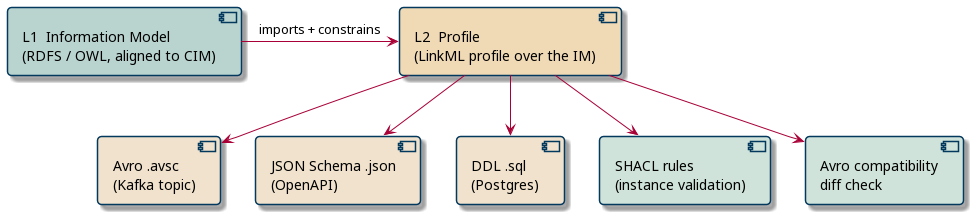
\includegraphics[width=\linewidth]{slides/exchange/consistency/figs/lifecycle.png}
		\end{column}
		\begin{column}{0.43\textwidth}
			\textbf{Consistency comes from the graph structure, not from discipline:}\\[0.4em]
			\begin{itemize}\scriptsize
				\item every artifact is \emph{downstream} of the profile
				\item a change to \texttt{PhaseCode} happens \emph{once} in the profile
				\item the validator is derived \emph{from} the same profile — one rule set
				\item review becomes: does this change the profile? what does it do to each artifact?
			\end{itemize}
		\end{column}
	\end{columns}

\end{frame}

\begin{frame}{The toolchain}
	\begin{itemize}
		\item \textbf{L1} \; \textbf{RDFS$/$OWL} — an aligned vocabulary (here CIM IEC 61970-301, with \texttt{owl:equivalentClass})
		\item \textbf{L2} \; a \textbf{LinkML profile} that imports the IM and narrows it \;$~\Rightarrow$~ \texttt{linkml-shacl} emits the conformance rules
		\item \textbf{L3} \; \texttt{linkml-avro}, \texttt{linkml-jsonschema}, \texttt{linkml-sql} — one command each, all from \emph{the same} profile
	\end{itemize}
	\vspace{0.3em}
	\begin{minipage}{0.99\linewidth}
	\lstinputlisting[style=code]{code/pipeline.sh}
	\end{minipage}
	\textbf{One profile. Three artifacts. One validator.}\\
	All of them \emph{generated} in the same CI job; none of them hand-edited.
\end{frame}


% \begin{frame}
% 	\frametitle{Data Uitwisseling}
% 	\begin{figure}
% 		\only<1>\includegraphics[width=0.4\textwidth]{}
% 		\only<2>\includegraphics[width=0.4\textwidth]{}
% 		\caption{Data Uitwisseling zonder je applicatie overhoop te gooien}
% 		\label{fig:data-uitwisseling}
% 	\end{figure}
% \end{frame}



\begin{frame}
  \frametitle{Data Uitwisseling}
  \begin{figure}
    \centering
    % First click – show the original picture
    \only<1>{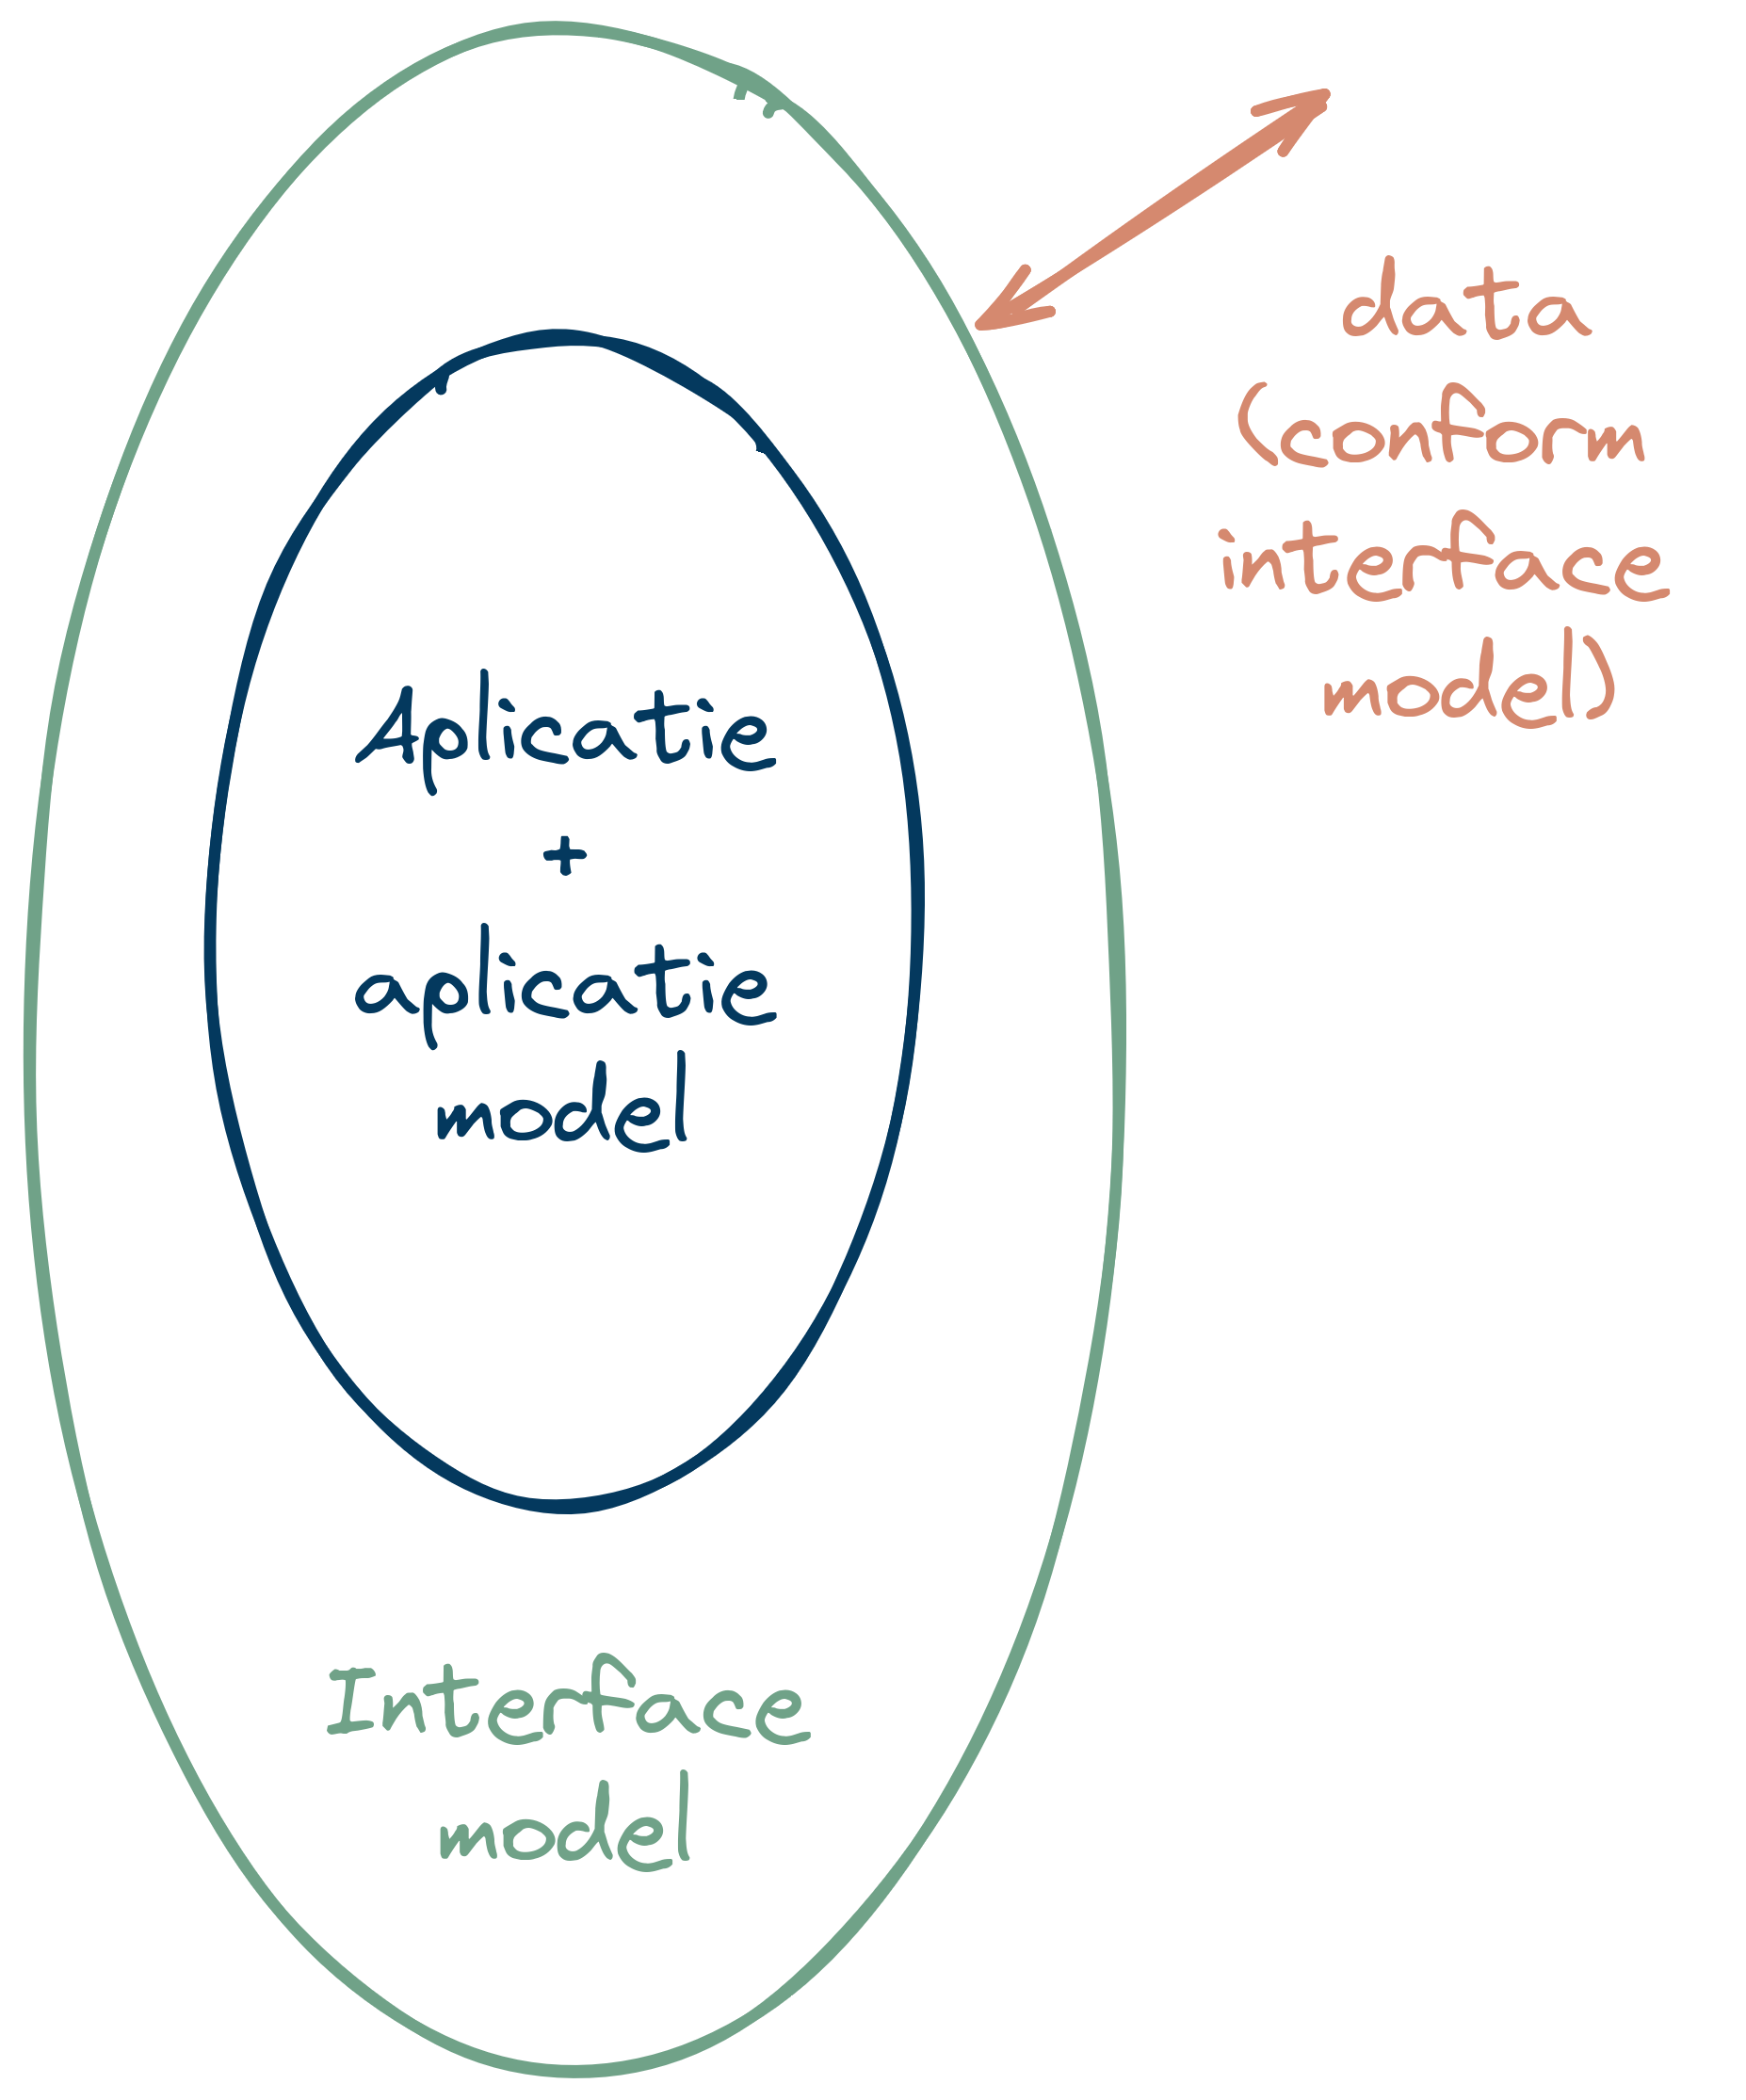
\includegraphics[height=0.5\textheight, keepaspectratio]{slides/exchange/data-uitwisseling/figs/data-uitwisseling.png}}
    % Second click – replace it with the second picture
    \only<2>{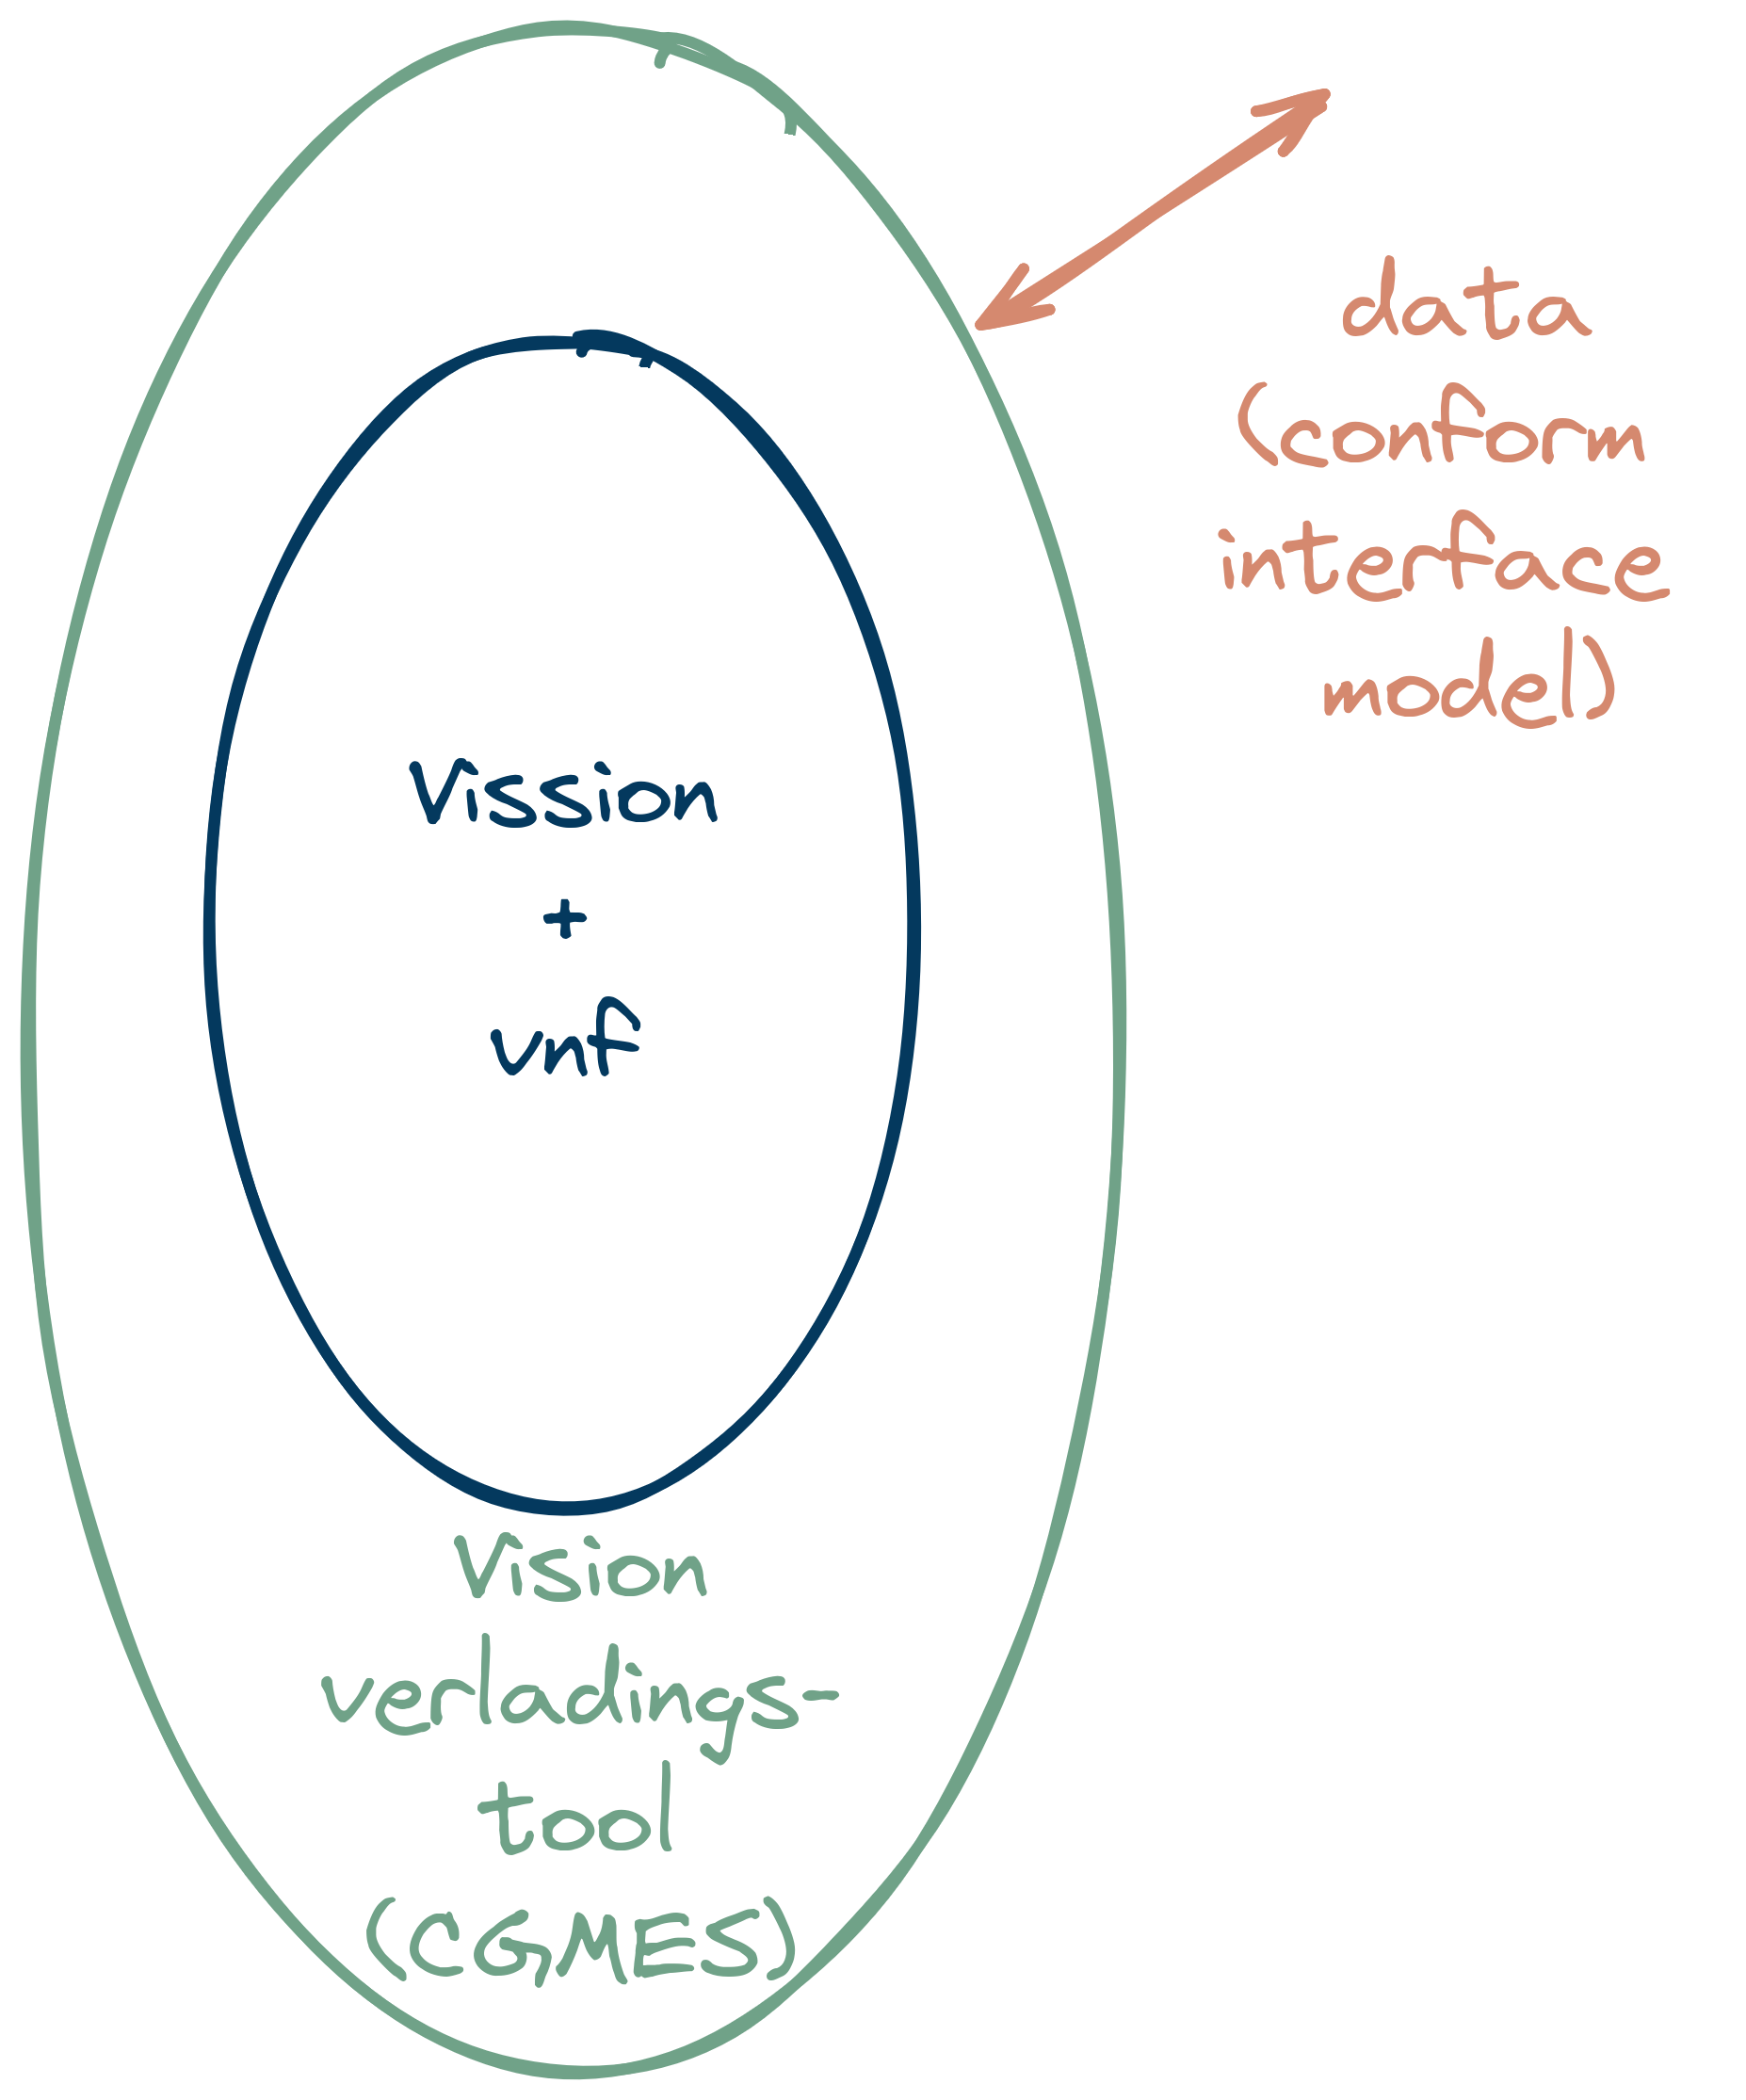
\includegraphics[height=0.5\textheight, keepaspectratio]{slides/exchange/data-uitwisseling/figs/data-uitwisseling-vision.png}}

    \caption{Data Uitwisseling zonder je applicatie overhoop te gooien}
    \label{fig:data-uitwisseling}
  \end{figure}
\end{frame}


\section{How Netbeheer Nederland manages profiles and schemas}
\begin{frame}
    \frametitle{CIM vs CGMES}
    \begin{figure}
        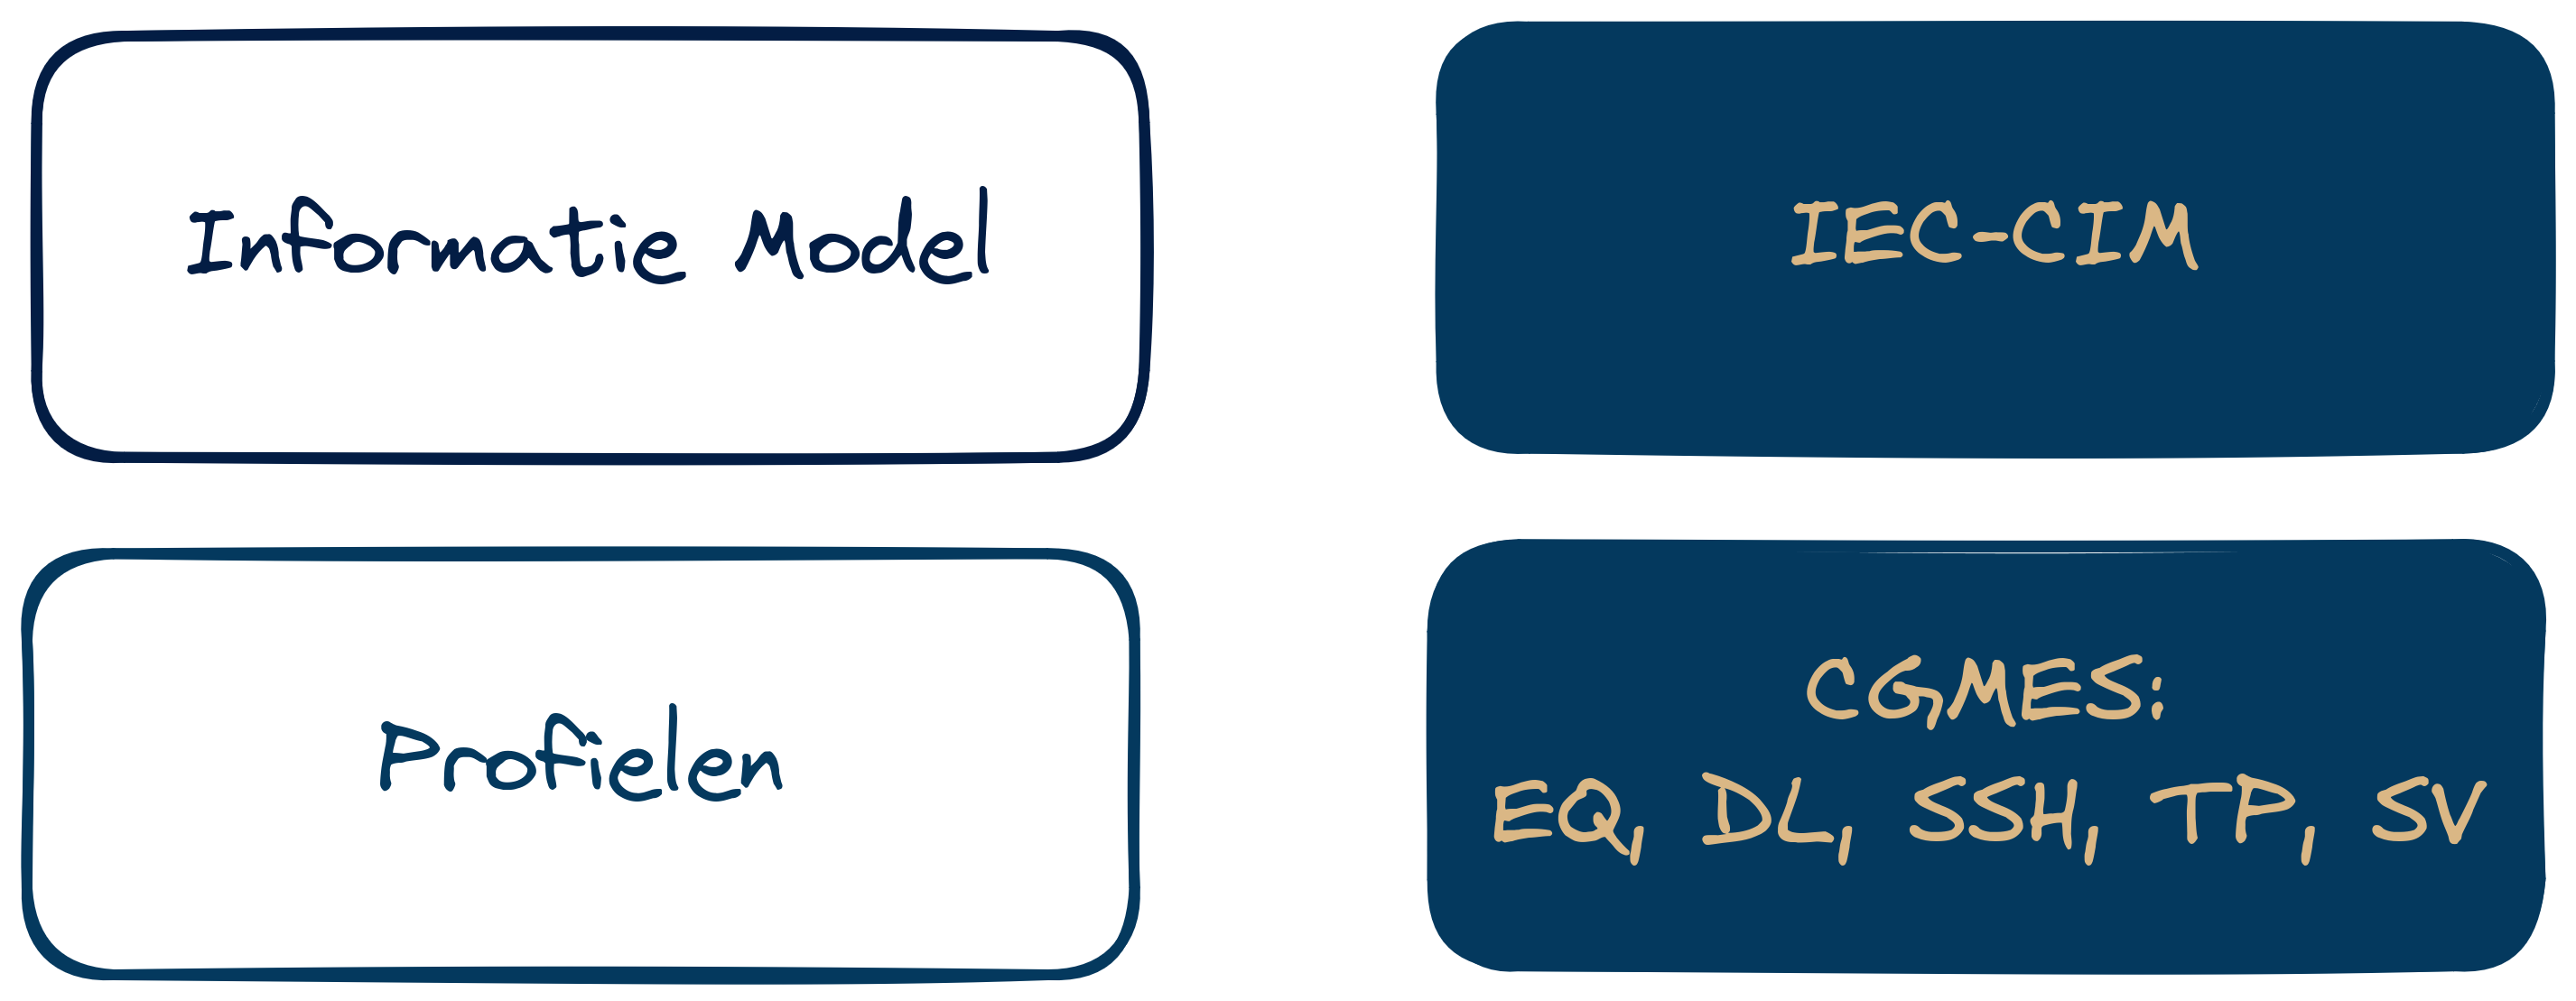
\includegraphics[width=0.6\textwidth]{slides/nbnl/cim-cgmes/figs/CIM-CGMES.png}
        \caption{Informatiemodellen en profielen}
        \label{fig:cim-cgmes}
    \end{figure}
\end{frame}
\begin{frame}
    \frametitle{Hoe de profielen samenhangen}
    \begin{figure}
        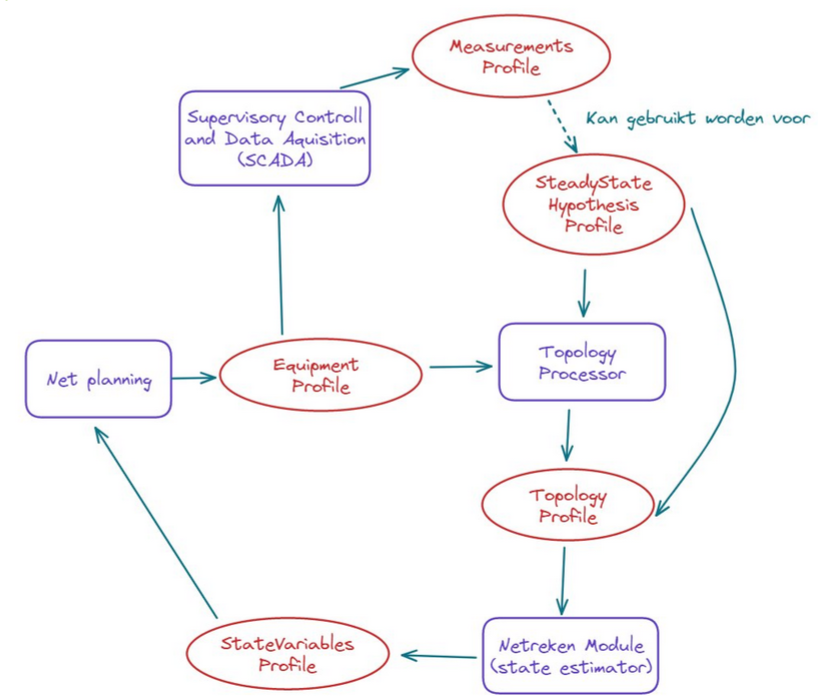
\includegraphics[height=0.55\textheight, keepaspectratio]{slides/nbnl/profiles-samenhang/figs/profiles-samenhang.png}
        \caption{Informatiemodellen en profielen}
        \label{fig:profiles-samenhang}
    \end{figure}
\end{frame}
\begin{frame}{How Netbeheer Nederland runs this in practice}
  \framesubtitle{Observations, not advice — check with your peers}
  \footnotesize
  \setlength{\itemsep}{0.5pt}
  \setlength{\parsep}{0pt}

  \begin{itemize}
    \item Netbeheer Nederland publishes \textbf{CGMES-based profiles} as the exchange language for grid data between DSOs and the TSO:
    \begin{itemize}
      \item documentation: \href{https://modellen.netbeheernederland.nl/cgmes/}{modellen.netbeheernederland.nl/cgmes}
      \item built on IEC 61970 CIM (the vocabulary) + ENTSO-E CGMES (the Dutch/European profile)
    \end{itemize}
    \pause
    \item The profile is \emph{use-case specific}: congestion calculation, capacity calculation, topology exchange — each is a closed-world subset of the open-world model.
    \pause
    \item The schemas (GML/RDF/XML artifacts) are \emph{derived} from the profile, not the other way round — same discipline as in our four-layer stack.
  \end{itemize}
\end{frame}

\begin{frame}{For DSOs in the Netherlands: the practical consequence}
  \footnotesize
  \setlength{\itemsep}{0.5pt}
  \setlength{\parsep}{0pt}

  \begin{itemize}
    \item your exchange \emph{must} be expressible in CIM terms, because the other side (TSO, other DSOs, market parties) is already there
    \item DER assets that want to be \emph{seen} in that exchange need a CIM representation — that is the gap this week closes.
  \end{itemize}

  \vspace{0.2cm}
  \begin{block}{Exercise (optional, in pairs)}
    List the artifacts your openADR flow already produces and mark which already have a CIM counterpart — and which don't.
  \end{block}
\end{frame}


\section{The yardstick, applied: openADR 3.0}
\begin{frame}{The standard as defined — what the yardstick applies to}

  \footnotesize
  \setlength{\itemsep}{4pt}
  \setlength{\parsep}{0pt}

  \begin{itemize}
    \item The \textbf{normative reference of OADR 3 is an OpenAPI document (YAML)}:
      the Alliance calls it ``the normative reference for OADR 3'', and it
      ``supersedes any statements made in other documentation''.
    \item The accompanying \textbf{``Definitions'' document} restates the same
      model in prose — and is, by that very clause, \emph{not} the normative one.
    \item What the standard defines is a \textbf{REST + JSON API}: paths,
      operations, and the payload schemas that move over it. Its predecessor
      (2.0b, SOAP/XML) has to be implemented alongside it.
  \end{itemize}

\end{frame}

% \begin{frame}{The normative artifact is a serialization of the model}
  \framesubtitle{What an OpenAPI YAML is — and what follows when it \emph{is} the standard}

  \begin{columns}[T]
    \begin{column}{0.44\textwidth}
      \textbf{What the artifact is}\\[0.3em]
      \begin{itemize}\scriptsize
        \item a description of \emph{one} HTTP API: paths, operations,
              parameters, security
        \item the payloads: \textbf{JSON Schemas} — \texttt{required},
              \texttt{type}, \texttt{range}, \texttt{enum}, nesting
        \item in the stack of this morning: \textbf{L3} — the serialization
        \vspace{0.25em}
        \item the format's only structural machinery: composition
              (\texttt{allOf}/\texttt{oneOf}), nesting, cross-references
              to other schemas
      \end{itemize}
    \end{column}
    \begin{column}{0.54\textwidth}
      \textbf{What follows when the standard is that}\\[0.3em]
      \begin{itemize}\scriptsize
        \item \textbf{Concepts live as payload schemas.} \texttt{Program},
              \texttt{Event}, \texttt{Reading}, \ldots are defined in the
              context of the messages they appear in. The format gives no
              concept identity, no inheritance, no disjointness — nothing
              another standard can reference or import
        \item \textbf{The model is bound to one serialization.} There is no
              \emph{normative} artifact that says what these concepts are,
              independent of HTTP + JSON
        \item \textbf{Two descriptions of the same model exist.} One
              normative (the YAML), one prose (``Definitions''). The
              standard's own rule when they differ: the YAML
              ``supersedes any statements made in other documentation''
      \end{itemize}
    \end{column}
  \end{columns}

  \vspace{0.25em}
  \begin{alertblock}{No verdict here}
    Nothing above is a reading of openADR against a goal — it is what
    follows, by construction, from the standard defining its normative
    artifact as a serialization. What that does to identity — and which
    of today's requirements apply to it — is the rest of this section.
  \end{alertblock}
\end{frame}

\begin{frame}{Instance data has no type}
  \framesubtitle{The validator checks \emph{structure} — not which thing a thing is}
  \begin{columns}[T]
    \begin{column}{0.49\textwidth}
      \textbf{What the validator has — one schema}\\[0.4em]
      \lstinputlisting[style=code, basicstyle=\ttfamily\tiny, columns=fullflexible]{code/equipment-schema.json}
    \end{column}
    \begin{column}{0.49\textwidth}
      \textbf{What arrives in the exchange — two instances}\\[0.4em]
      \lstinputlisting[style=code, basicstyle=\ttfamily\tiny, columns=fullflexible]{code/equipment-instances.json}
      \vspace{0.2em}
      \small The first is a \emph{Substation}; the second a \emph{Transformer}.
      The payload never says which — only the sender knows.
    \end{column}
  \end{columns}
  \vspace{0.4em}
  \small
  \textbf{The verdict:} both instances validate \alert{$\checkmark$} —
  including the Transformer, where a Substation was expected.
  The validator can only check that the structure matches, so it cannot decide
  which \emph{type} the data represents. The one that should not pass,
  \alert{passes}.
\end{frame}

% \begin{frame}{A serialization cannot be a model}
  \framesubtitle{What the standard adds to name a type — and what it still cannot do}
  \begin{columns}[T]
    \begin{column}{0.53\textwidth}
      \textbf{The serialization's answer: a \texttt{type} string}\\[0.4em]
      \lstinputlisting[style=code, basicstyle=\ttfamily\tiny, columns=fullflexible]{code/type-tag.yaml}
      \vspace{0.2em}
      \small The discriminator reads the \texttt{"type"} tag the sender writes —
      it picks a schema; it does not make the data typed.
    \end{column}
    \begin{column}{0.47\textwidth}
      \textbf{What stays out of reach}\\[0.4em]
      \begin{itemize}\scriptsize
        \item no concept identity: a \texttt{\$defs} entry is a named \emph{schema}, not a kind the value \emph{is} — nothing other standards can reference or align to (no \texttt{owl:equivalentClass} hook)
        \item no inheritance, no disjointness, no reasoning
        \item closed \& positional: \emph{extending} a kind = forking the schema
        \item in a typed model the instance \emph{is} a Substation — and SHACL can require that (\texttt{shacl:class})
      \end{itemize}
    \end{column}
  \end{columns}
  \vspace{0.2em}
  \begin{alertblock}{So the layers stay where they belong}
    \small Meaning + type-level validation $\Rightarrow$ RDFS/OWL + SHACL;
    serialization $\Rightarrow$ JSON Schema / Avro / SQL.
    OADR 3's normative core is exactly this — the serialization promoted to
    the model (Req.\ \ref{req:universal}).
  \end{alertblock}
\end{frame}

\begin{frame}{openADR 3.0 against the three requirements}
  \framesubtitle{The requirements as defined earlier in this deck — the standard as defined}

  \scriptsize
  \setlength{\tabcolsep}{5pt}
  \renewcommand{\arraystretch}{1.35}
  \begin{center}
  \begin{tabular}{@{}p{3.2cm}p{11.8cm}@{}}
    \rowcolor[HTML]{031d44}
    {\color{white}\textbf{Requirement}} &
    {\color{white}\textbf{openADR 3.0}}\\
    \midrule
    \textbf{Req.\ \ref{req:universal}}\\ \textit{serves multiple use cases} &
      Use cases enter as \textbf{profiles} — slices of the API surface — and
      certification is \textbf{per profile}. The content shared between use
      cases is the payload schemas of the normative YAML: shared
      \emph{as an artifact}, not as concepts that can be referenced or
      imported on their own. \emph{This seems to work!}\\
    \textbf{Req.\ \ref{req:technology}}\\ \textit{not technology-specific} &
      OADR 3 is defined as a \textbf{REST + JSON API}; the model content
      sits inside that description of the transport. The predecessor
      already marks the pattern: 2.0b (SOAP/XML) and 3.0 (REST/JSON) are
      two serializations for the same subject matter, each with its own normative
      description. So openADRm in is current form, is not technology agnostic.\\
    \textbf{Req.\ \ref{req:consistent}}\\ \textit{no empty sets} &
      JSON schema classes do not define mathematical sets, \emph{this is cannot be validated.} \\
    
    \bottomrule
  \end{tabular}
  \end{center}

  \vspace{0.2cm}
  \begin{center}
  {\footnotesize The table describes the standard against the requirements.
  It makes no proposal and offers no remediation.}
  \end{center}
\end{frame}


\section{Takeaways}
\begin{frame}{Takeaways — Day 1}

  \setlength{\itemsep}{2.5pt}
  \setlength{\parsep}{0pt}

  \begin{enumerate}
    \item \textbf{Defining an information standard}
    \begin{itemize}
      \item interoperability is a community quality; a standard is what they decide to make \emph{testable}
    \end{itemize}
    \pause
    \item \textbf{The best practice stack}
    \begin{itemize}
      \item L0 concepts (SKOS) $\rightarrow$ L1 open-world vocabulary $\rightarrow$ L2 profile $\rightarrow$ L3 \emph{derived} artifacts; schema $\neq$ meaning
      \item MOF: choose a pivot model, don't chase one; validate from the profile (SHACL)
      \item proven in practice: Netbeheer Nederland runs this with CIM/CGMES
    \end{itemize}
    \pause
    \item \textbf{openADR 3.0 through that lens}
    \begin{itemize}
      \item the normative core of the standard is a \emph{serialization}: the OpenAPI YAML,
            with the model defined inside it
      \item the three requirements of the day attach to exactly that choice:
            multiple use cases, technology-independence, no empty sets
    \end{itemize}
  \end{enumerate}
\end{frame}

\begin{frame}{Conclusion}

    \begin{itemize}
        \item A well-defined information standard facilitates both organization-wide and inter-organization data management
        \begin{itemize}
            \item It allows the use of expert models for \textit{every} domain
            \item Standardization of information helps with every aspect of (FAIR) data management
        \end{itemize}
        \item Defining and standardizing information is about standardizing standards
        \begin{itemize}
            \item The motivations are identical
            \item The methods are identical
            \item Just one level of abstraction higher
        \end{itemize}
        \item A well-defined information standard requires
        \begin{itemize}

            \item A clear distinction between vocabulary models and constraint models (req. 1)
            \item Harmonized metamodels; choosing an appropriate pivot model is key (req. 2)
            \item A fair amount of interpretation, but an upper ontology can provide a structure for interpretation (req. 3)
        \end{itemize}
        \item Applied to openADR 3.0: what the standard makes normative is the \emph{serialization} of the model
        — the OpenAPI document — and the requirements of the day apply to that artifact directly
        %\item Most of what I have discussed today is at best in the experimental phase, so there is a lot of work to be done \pause (and yes, I think EPRI might have a role in that)
    \end{itemize}
\end{frame}

\begin{frame}{Day 2: CIM, IEC 61850, the DSO and the DER}
  \small

  \begin{multicols}{2}
    \begin{itemize}
      \item CIM and 61850 in the SGAM context — and what that relationship teaches openADR
      \item The origins of CIM
      \item CIM and \emph{netrekenen}: why the grid is calculated, not just managed
      \item Kirchhoff's law, and the four things to exchange to be able to calculate:
      \begin{itemize}
        \item Connectivity
        \item Topology
        \item State
        \item Results
      \end{itemize}
    \end{itemize}
  \end{multicols}
  \vspace{0.2cm}
  \begin{multicols}{2}
    \begin{itemize}
      \item What a \textbf{bedrijfsvoeringscentrum} must know about a charging point to be able to steer it well
      \item When CIM is interesting for openADR — and honestly, when it is not
      \item CIM: the good parts, the rough parts, and the pitfalls
      \item Object-oriented or semantic — and what that means for your models
      \item CIM and OpenAPI
      \item Standards to keep in your gate: SOSA/SSN, QU, and metadata standards
    \end{itemize}
  \end{multicols}
\end{frame}


\section{Q \& A}
\begin{frame}{Thank you — questions?}

\vspace{0.5cm}
\begin{center}
    {\large \href{mailto:joep@uuidea.eu}{joep@uuidea.eu}}\\[1em]
    % {\large \href{https://uuidea.eu}{www.uuidea.eu}}\\[1em]
    {\large GitHub: \href{https://github.com/uuidea}{github.com/uuidea}}
\end{center}

\vspace{0.5cm}
\begin{center}
\small Content shared under \href{https://creativecommons.org/licenses/by-sa/4.0/}{CC BY-SA 4.0}
\end{center}

\end{frame}


\end{document}
